
\section{Overview}

Despite the massive success brought by neural machine translation~\citep[NMT,][]{sutskever2014sequence,bahdanau2014neural,vaswani2017attention}, it has been noticed that the vanilla NMT often lags behind conventional machine translation systems, such as statistical phrase-based translation systems~\citep[PBMT,][]{koehn2003statistical}, for low-resource language pairs~\citep[see, e.g.,][]{koehn2017six}. In the past few years, various approaches have been proposed to address this issue. The first attempts at tackling this problem exploited the availability of monolingual corpora~\citep{Gulcehre-Orhan-et-al-2015,sennrich2015improving,zhang2016exploiting}. It was later followed by approaches based on multilingual translation, in which the goal was to exploit knowledge from high-resource language pairs by training a single NMT system on a mix of high-resource and low-resource language pairs~\citep{firat2016multi,firat2016zero,lee2016fully,johnson2016google,ha2016toward}. Its variant, transfer learning, was also proposed by \citet{zoph2016transfer}, in which an NMT system is pretrained on a high-resource language pair before being finetuned on a target low-resource language pair.

In this chapter, we follow up on these latest approaches based on multilingual NMT and propose a meta-learning algorithm for low-resource neural machine translation. We start by arguing that the recently proposed model-agnostic meta-learning algorithm~\citep[MAML,][]{finn2017model} could be applied to low-resource machine translation by viewing language pairs as separate tasks. This view enables us to use MAML to find the initialization of model parameters that facilitate fast adaptation for a new language pair with a minimal amount of training examples (\textsection\ref{cp6.sec.maml-mt}). Furthermore, the vanilla MAML however cannot handle tasks with mismatched input and output. We overcome this limitation by incorporating the universal lexical representation (ULR) introduced in the previous chapter, and adapting it for the meta-learning scenario (\textsection\ref{cp6.sec.ulr}).

We extensively evaluate the effectiveness and generalizing ability of the proposed meta-learning algorithm on low-resource neural machine translation. We utilize 17 languages from Europarl and Russian from WMT as the source tasks and test the meta-learned parameter initialization against five target languages (Ro, Lv, Fi, Tr and Ko), in all cases translating to English. Our experiments using only up to 160k tokens in each of the target task reveal that the proposed meta-learning approach outperforms the multilingual translation approach across all the target language pairs, and the gap grows as the number of training examples decreases.



\section{Background: Meta-Learning}
% \subsection{Low-Resource Neural Machine Translation}
%\paragraph{Neural Machine Translation (NMT)}
%Given a source sentence $X=\{x_1, ..., x_{T'}\}$, a neural machine translation model factors the distribution over possible output sentences $Y=\{y_1, ..., y_T\}$ into a chain of conditional probabilities with a left-to-right causal structure:
%\begin{equation}
%p(Y|X; \theta) = \prod_{t=1}^{T+1} p(y_t| y_{0:t-1}, x_{1:T'}; \theta),
%\end{equation}
%where special tokens $y_0$ ($\langle \mathrm{bos}\rangle$) and $y_{T+1}$ ($\langle \mathrm{eos}\rangle$) are used to represent the beginning and the end of a target sentence.
%These conditional probabilities are parameterized using a neural network. Typically, an encoder-decoder architecture~\citep{sutskever2014sequence,Cho2014a,bahdanau2014neural} with a RNN-based decoder is used. More recently, architectures without any recurrent structures~\citep{gehring2017convolutional,vaswani2017attention} have been proposed and shown to speedup training while achieving state-of-the-art performance.





%\paragraph{Meta Learning}

In the machine learning community, meta-learning, or learning-to-learn, has recently received interests. Meta-learning tries to solve the problem of “fast adaptation on new training data.”  One of the most successful applications of meta-learning has been on few-shot (or one-shot) learning~\citep{lake2015human}, where a neural network is trained to readily learn to classify inputs based on only one or a few training examples. There are two categories of meta-learning:
\begin{enumerate}
    \item learning a meta-policy for updating model parameters~\citep[see, e.g.,][]{andrychowicz2016learning,ha2016hypernetworks,mishra2017meta}.
    \item  learning a good parameter initialization for fast adaptation~\citep[see, e.g.,][]{finn2017model,vinyals2016matching,snell2017prototypical}. 
\end{enumerate}
In this chapter, we propose to use a meta-learning algorithm for low-resource neural machine translation based on the second category. More specifically, we extend the idea of model-agnostic meta-learning~\citep[MAML,][]{finn2017model} in the multilingual scenario.

% KC: unnecessary here. we will explain the method in detail right below.
% Take the latter as an example, it can be summarized as repeating the following two steps: (1) simulate an episode by sampling a small amounts of training data and “train” a model starting from the meta-model; (2) based on evaluation of the “trained” model, update the meta-model. The ultimate goal of meta-learning and few-shot learning is the same for the case of low resource translation, but there is hardly any work investigating meta-learning for sequence generation tasks such as machine translation. 




\section{Meta-Learning for Extremely Low-Resource Neural Machine Translation}
\label{cp6.sec.maml-mt}

The underlying idea of MAML is to use a set of source tasks $\left\{ \mathcal{T}^1, \ldots, \mathcal{T}^K \right\}$ to find the initialization of parameters $\theta^0$ from which learning a target task $\mathcal{T}^0$ would require only a small number of training examples. In the context of machine translation, this amounts to using many high-resource language pairs to find good initial parameters and training a new translation model on a low-resource language starting from the found initial parameters. This process can be understood as 
\begin{align}
\theta^* = \text{Learn}(\mathcal{T}^0; \text{MetaLearn}(\mathcal{T}^1, \ldots, \mathcal{T}^K)).
\end{align}
That is, we {\it meta-learn} the initialization from auxiliary tasks and continue to {\it learn} the target task. We refer the proposed meta-learning method for NMT to MetaNMT.
See Fig.~\ref{cp6.fig.framework} for the overall illustration. 
\begin{sidewaysfigure}[hptb]
    \centering
    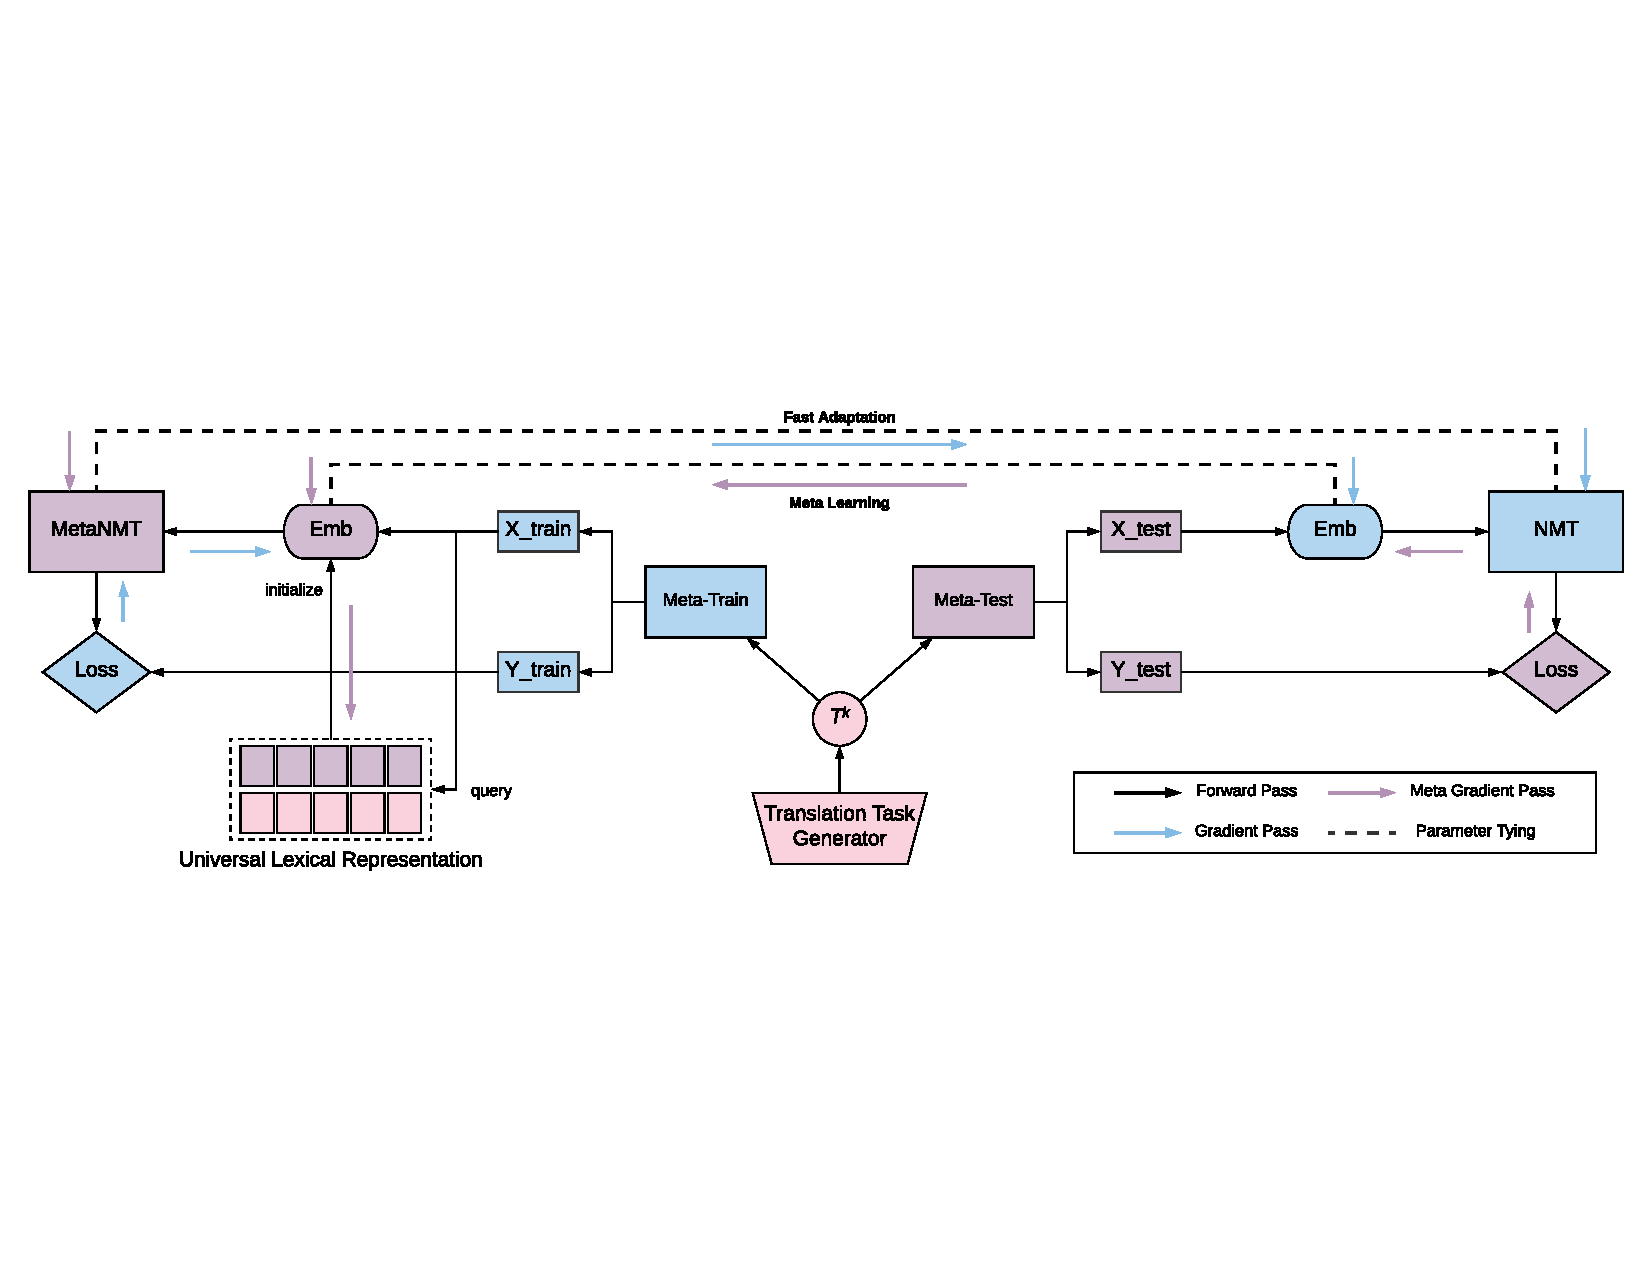
\includegraphics[width=\linewidth]{figs/meta/framework.pdf}
    \caption{The graphical illustration of the training process of the proposed MetaNMT. For each episode, one task (language pair) is sampled for meta-learning. The boxes and arrows in blue are mainly involved in language-specific learning (\textsection\ref{cp6.sec.lsl}), and those in purple in meta-learning (\textsection\ref{cp6.sec.ml}).}
    \label{cp6.fig.framework}
\end{sidewaysfigure}


\subsection{Learn: language-specific learning}
\label{cp6.sec.lsl}
Given any initial parameters $\theta^0$ (which can be either random or meta-learned), 
%We use the meta-learned initial parameters $\theta^0$ to 
the prior distribution of the parameters of a desired NMT model can be defined %a prior distribution over the model parameters 
as an isotropic Guassian:
\begin{align}
    \theta_i \sim \mathcal{N}(\theta^0_i, 1/\beta^2),
\end{align}
where $1/\beta$ is a variance. With this prior distribution, we formulate the language-specific learning process $\text{Learn}(D_\mathcal{T}; \theta^0)$ as maximizing the log-posterior of the model parameters given data $D_{\mathcal{T}}$:
\begin{equation}
	\begin{split}
    &\text{Learn}(D_\mathcal{T}; \theta^0) = 
    \arg\max_{\theta} \mathcal{L}^{D_\mathcal{T}} (\theta)
    \\
    &=\arg\max_{\theta}\!\!\!\!
    \sum_{(X,Y) \in D_{\mathcal{T}}} \!\! \!\!
    \log p(Y | X, \theta)  
    - \beta \| \theta - \theta^0 \|^2,
\end{split}
\end{equation}
where we assume $p(X|\theta)$ to be uniform. 
The first term above corresponds to the maximum likelihood criterion often used for training a usual NMT system. The second term discourages the newly learned model from deviating too much from the initial parameters, alleviating the issue of over-fitting when there is not enough training data. In practice, we solve the problem above by maximizing the first term with gradient-based optimization and early-stopping after only a few update steps. Thus, in the low-resource scenario, finding a good initialization $\theta^0$ strongly correlates the final performance of the resulting model.


\subsection{MetaLearn}
\label{cp6.sec.ml}

We find the initialization $\theta^0$ by repeatedly simulating low-resource translation scenarios using auxiliary, high-resource language pairs. Following \citet{finn2017model} 
%and \citet{al2017continuous}, 
we achieve this goal by defining the meta-objective function as
% \begin{align}
% \label{cp6.eq.meta}
%     \mathcal{L}(\theta) =& 
%     \mathbb{E}_{k,k'} \mathbb{E}_{D_{\mathcal{T}^{k}},D_{\mathcal{T}^{k'}}} \\
%     &\left[
%     \sum_{(X,Y) \in D_{\mathcal{T}^{k'}}} \!\!\!\!\!
%     \log p(Y|X; \text{Learn}(D_{\mathcal{T}^{k}}; \theta))
%     \right], \nonumber
% \end{align}
\begin{align}
\label{cp6.eq.meta}
    \mathcal{L}(\theta) =
    \mathbb{E}_{k} \mathbb{E}_{D_{\mathcal{T}^{k}}, D'_{\mathcal{T}^{k}}} 
    \left[
    \sum_{(X,Y) \in D'_{\mathcal{T}^{k}}} \!\!\!\!\!\!\!
    \log p(Y|X; \text{Learn}(D_{\mathcal{T}^{k}}; \theta))
    \right],
\end{align}
%where $k',k \!\sim\!\mathcal{U}(\left\{1, \ldots, K \right\})$, and $D_{\mathcal{T}}$ follows a uniform distribution over the power set of $\mathcal{T}$.  
where $k \!\sim\!\mathcal{U}(\left\{1, \ldots, K \right\})$ refers to one meta-learning episode, and $D_{\mathcal{T}}$,  $D'_{\mathcal{T}}$ follow the uniform distribution over $\mathcal{T}$'s data.  

We maximize the meta-objective function using stochastic approximation~\citep{robbins1951stochastic} with gradient descent. For each episode, we uniformly sample one source task at random, $\mathcal{T}^{k}$. %and $\mathcal{T}^{k'}$. 
We then sample two subsets of training examples independently from the chosen task, $D_{\mathcal{T}^{k}}$ and $D'_{\mathcal{T}^{k}}$. We use the former to {\it simulate} language-specific learning and the latter to {\it evaluate} its outcome. 
%and $D_{\mathcal{T}^{k'}}$. We use the first one to {\it simulate} learning and the latter to {\it evaluate} its outcome. 
Assuming a single gradient step is taken only the with learning rate $\eta$,
% without loss of generality, 
the simulation is:
\begin{align}
    \theta'_k = \text{Learn}(D_{\mathcal{T}^k}; \theta) =
    \theta - \eta \nabla_{\theta} \mathcal{L}^{D_{\mathcal{T}^k}}(\theta).
\end{align}
Once the simulation of learning is done, we evaluate the updated parameters $\theta'_k$ on $D'_{\mathcal{T}^{k}}$, %$D_{\mathcal{T}^{k'}}$, 
%i.e., $\mathcal{L}^{D'_{\mathcal{T}^{k}}}(\theta'_k)$. 
The gradient computed from this evaluation, which we refer to as {\it meta-gradient}, is used to update the meta model $\theta$. It is possible to aggregate multiple episodes of source tasks before updating $\theta$:
\begin{align}
    \theta \leftarrow \theta - \eta' \sum_k \nabla_\theta \mathcal{L}^{D'_{\mathcal{T}^{k}}}(\theta'_k),
\end{align}
where $\eta'$ is the meta learning rate. 

Unlike a usual learning scenario, the resulting model $\theta^0$ from this meta-learning procedure is not necessarily a good model on its own. It is however a good starting point for training a good model using only a few steps of learning. In the context of machine translation, this procedure can be understood as finding the initialization of a neural machine translation system that could quickly adapt to a new language pair by simulating such a fast adaptation scenario using many high-resource language pairs. 



\paragraph{Meta-Gradient}

% KC: it is not intractable, if we use R-op from Pearlmutter.
% It is intractable to compute the meta-gradient, which requires computing the Hessian matrix, exactly in practice for a usual NMT system which often contains tens of millions of parameters. Instead, 
We use the following approximation property 
\begin{equation}
H(x)v \approx \frac{\nabla(x+\nu v) - \nabla(x)}{\nu}
\end{equation}
to approximate the meta-gradient:\footnote{We omit the subscript $k$ for simplicity.}
\begin{equation}
\begin{split}
	  &\nabla_\theta  \mathcal{L}^{D'}(\theta') = \nabla_{\theta'} \mathcal{L}^{D'}(\theta') 
    \nabla_{\theta}(\theta - \eta \nabla_{\theta} \mathcal{L}^{D}(\theta)) \\
    &= \nabla_{\theta'} \mathcal{L}^{D'}(\theta')
    - \eta \nabla_{\theta'} \mathcal{L}^{D'}(\theta') H_{\theta}(\mathcal{L}^{D}(\theta)) \\
    &\approx 
    \nabla_{\theta'} \mathcal{L}^{D'}(\theta')
    - \frac{\eta}{\nu} \left[
    \nabla_{\theta}\mathcal{L}^D(\theta)\bigg|_{\hat{\theta}}
    - \nabla_{\theta}\mathcal{L}^D(\theta)\bigg|_{\theta} 
    \right],
\end{split}
\end{equation}
% \begin{align*}
%     \nabla_\theta & \mathcal{L}^{D'}(\theta'_k) = \nabla_{\theta'_k} \mathcal{L}^{k'}(\theta'_k) 
%     \nabla_{\theta}(\theta - \eta \nabla_{\theta} \mathcal{L}^{k}(\theta)) \\
%     &= \nabla_{\theta'_k} \mathcal{L}^{k'}(\theta'_k)
%     - \eta \nabla_{\theta'_k} \mathcal{L}^{k'}(\theta'_k) H_{\theta}(\mathcal{L}^{k}(\theta)) \\
%     &\approx 
%     \nabla_{\theta'_k} \mathcal{L}^{k'}(\theta'_k)
%     - \frac{\eta}{\nu} \left(
%     \nabla_{\theta_k}\mathcal{L}^k(\hat{\theta}_k) 
%     - \nabla_{\theta_k}\mathcal{L}^k(\theta_k) 
%     \right),
% \end{align*}
where $\nu$ is a small constant and 
\begin{equation}
	\hat{\theta} = \theta + \nu \nabla_{\theta'}\mathcal{L}^{D'}(\theta').	
\end{equation}

In practice, we find that it is also possible to ignore the second-order term, ending up with the following simplified update rule:
\begin{align}
\label{cp6.eq.meta-grad-first}
    \nabla_\theta \mathcal{L}^{D'}(\theta') \approx
    \nabla_{\theta'} & \mathcal{L}^{D'}(\theta').
\end{align}
%We test both later in the experiments. 




% \alert{KC: TODO}



% \subsection{Fast Adaptation}
% % \paragraph{NMT in an Inference Perspective}
% We focus on finding an optimal neural machine translation system $\theta^*$ which performs well on a new unseen translation pair $\mathcal{T}^0$ with a small number training examples only. One general view is to cast learning of an NMT model $\theta^*$ as maximizing the conditional posterior given the whole training examples:
% \begin{align}
%     \label{eq.learn}
%     %\begin{split}
%     &\text{Learn}(\mathcal{T}^0; \theta^0) \nonumber = \argmax_{\theta} \sum_{X, Y}^{\mathcal{T}^0}\log p(\theta|Y, X)  \\
%     & = \argmax_{\theta} \sum_{X, Y}^{\mathcal{T}^0}\log p(Y | X; \theta) - \beta\cdot \|\theta - \theta^0\|^2 %\nonumber
%     %\end{split}
% \end{align}
% where the first term is the conditional likelihood function, and the second term models the prior of the model. We use $\theta^0$ to denote an initial model. 
% Note that, the first term has a sum over the parallel sentences and dominates the objective as the size of the training examples grows,
% which is the typical MLE objective for training an NMT model. 

% Naive MLE training overfits and does not generalize with low-resource translation. We avoid it by penalizing the model to move too far away from the initial model $\theta^0$. In practise, we implement it implicitly by training the NMT model with the normal MLE objective, while performing early stopping in a small number of gradient steps. 

% \subsection{Meta Learning}
% % \paragraph{Two-step Process}
% Finding an adequate initial model $\theta^0$ highly affects the performance of the resulted final model $\theta^*$. Inspired from previous works~\citep{zoph2016transfer,firat2016multi,lee2016fully,johnson2016google,gu2018universal}, such initialization can be learned over a set of auxiliary multilingual translation pairs $\mathcal{T}^1, ..., \mathcal{T}^K$. As noted by \newcite{finn2017model}, meta-learning is the principal way of learning a good initialization that can quickly adapt to translation of new languages with only a few training examples. It makes much sense for us to recast the learning of Low-Resource NMT as a ``\textit{Meta-Learn $\rightarrow$ Learn}'' process. That is to say,
% \begin{equation}
%     \theta^* = \text{Learn}(\mathcal{T}^0; \text{MetaLearn}(\mathcal{T}^1, ...,\mathcal{T}^K))
% \end{equation}



% \paragraph{Meta Objective}
% Similar to  MAML~\citep{finn2017model}, the initial NMT model $\theta^0$ can be found by repeatedly ``simulating'' a low-resource (Eq.~\ref{eq.learn}) using a set of high-resource translation pairs. Assume that we have $K$ auxiliary pairs $\mathcal{T}^1, ..., \mathcal{T}^K$, our meta-objective for learning a good initialization model $\theta^0$ is:
% \begin{equation}
%     \label{eq.meta}
%     \max_{\theta} \sum_{k=1}^K \sum_{X, Y}^{\mathcal{T}^k} \log p(Y|X; \text{Learn}(\mathcal{T}^k; \theta))
% \end{equation}
% % \begin{equation}
% %     \label{eq.meta}
% %     \begin{split}
% %         &\max_{\theta} \mathbb{E}_k \left[\mathcal{L}^k(\theta')\right] = \\ 
% %         &\mathbb{E}_k \mathbb{E}_{X, Y \sim \mathcal{T}^k} \left[\log p(Y|X; \text{Learn}(\mathcal{T}^k; \theta))\right]
% %     \end{split}
% % \end{equation}
% where we denote $\theta'_k=\text{Learn}(\mathcal{T}^k; \theta)$ as the updated network in the inner-loop which corresponds to simulating low-resource translation sentences by randomly sampling a small fraction of the original dataset and performing only a small number of gradient steps over the sampled data to update the model. The language specific loss $\mathcal{L}^k_{\theta'_k}$ are then computed on a new set of examples from the same language pair with the updated parameters.

% Intuitively, as the same $\theta$ is shared by all the language pairs, the meta-objective implicitly forces the model to learn an initialization which is (1) near language-independent and (2) easy to adapt to new languages. 



% First, sample

% \paragraph{Objective}
% \begin{equation}
%     \max_{\theta} \mathbb{E}_{\mathcal{D}^{\text{train}} \sim W^0} \mathcal{L}^{\text{in}}\left(\mathcal{D}^{\text{train}}; \theta \right),
% \end{equation}

% \begin{equation}
%     \max_{\theta} \mathbb{E}_k \mathbb{E}_{\mathcal{D}^{\text{train}}, \mathcal{D}^{\text{test}} \sim W^k} \mathcal{L}^{\text{out}}\left(\mathcal{D}^{\text{test}}; \theta + \Delta(\mathcal{D}^{\text{train}}; \theta)  \right),
% \end{equation}






\paragraph{Related Work: Multilingual Transfer Learning}

The proposed MetaNMT differs from the existing framework of multilingual translation~\citep{lee2016fully,johnson2016google,gu2018universal} or transfer learning~\citep{zoph2016transfer}. The latter can be thought of as solving the following problem:
\begin{align}
    \max_{\theta} \mathcal{L}^{\text{multi}}(\theta) = \mathbb{E}_k\left[
    \sum_{(X,Y) \in D_k} \log p(Y|X; \theta)
    \right],
\end{align}
where $D_k$ is the training set of the $k$-th task, or language pair. The target low-resource language pair could either be a part of joint training or be trained separately starting from the solution $\theta^0$ found from solving the above problem. 

The major difference between the proposed MetaNMT and these multilingual transfer approaches is that the latter do not consider how learning happens with the target, low-resource language pair. The former explicitly incorporates the learning process within the framework by simulating it repeatedly in Eq.~\eqref{cp6.eq.meta}. As we will see later in the experiments, this results in a substantial gap in the final performance on the low-resource task. 

\paragraph{Illustration}
\begin{figure*}[hptb]
%\sidebysidecaption{0.76\linewidth}{0.23\linewidth}{%
    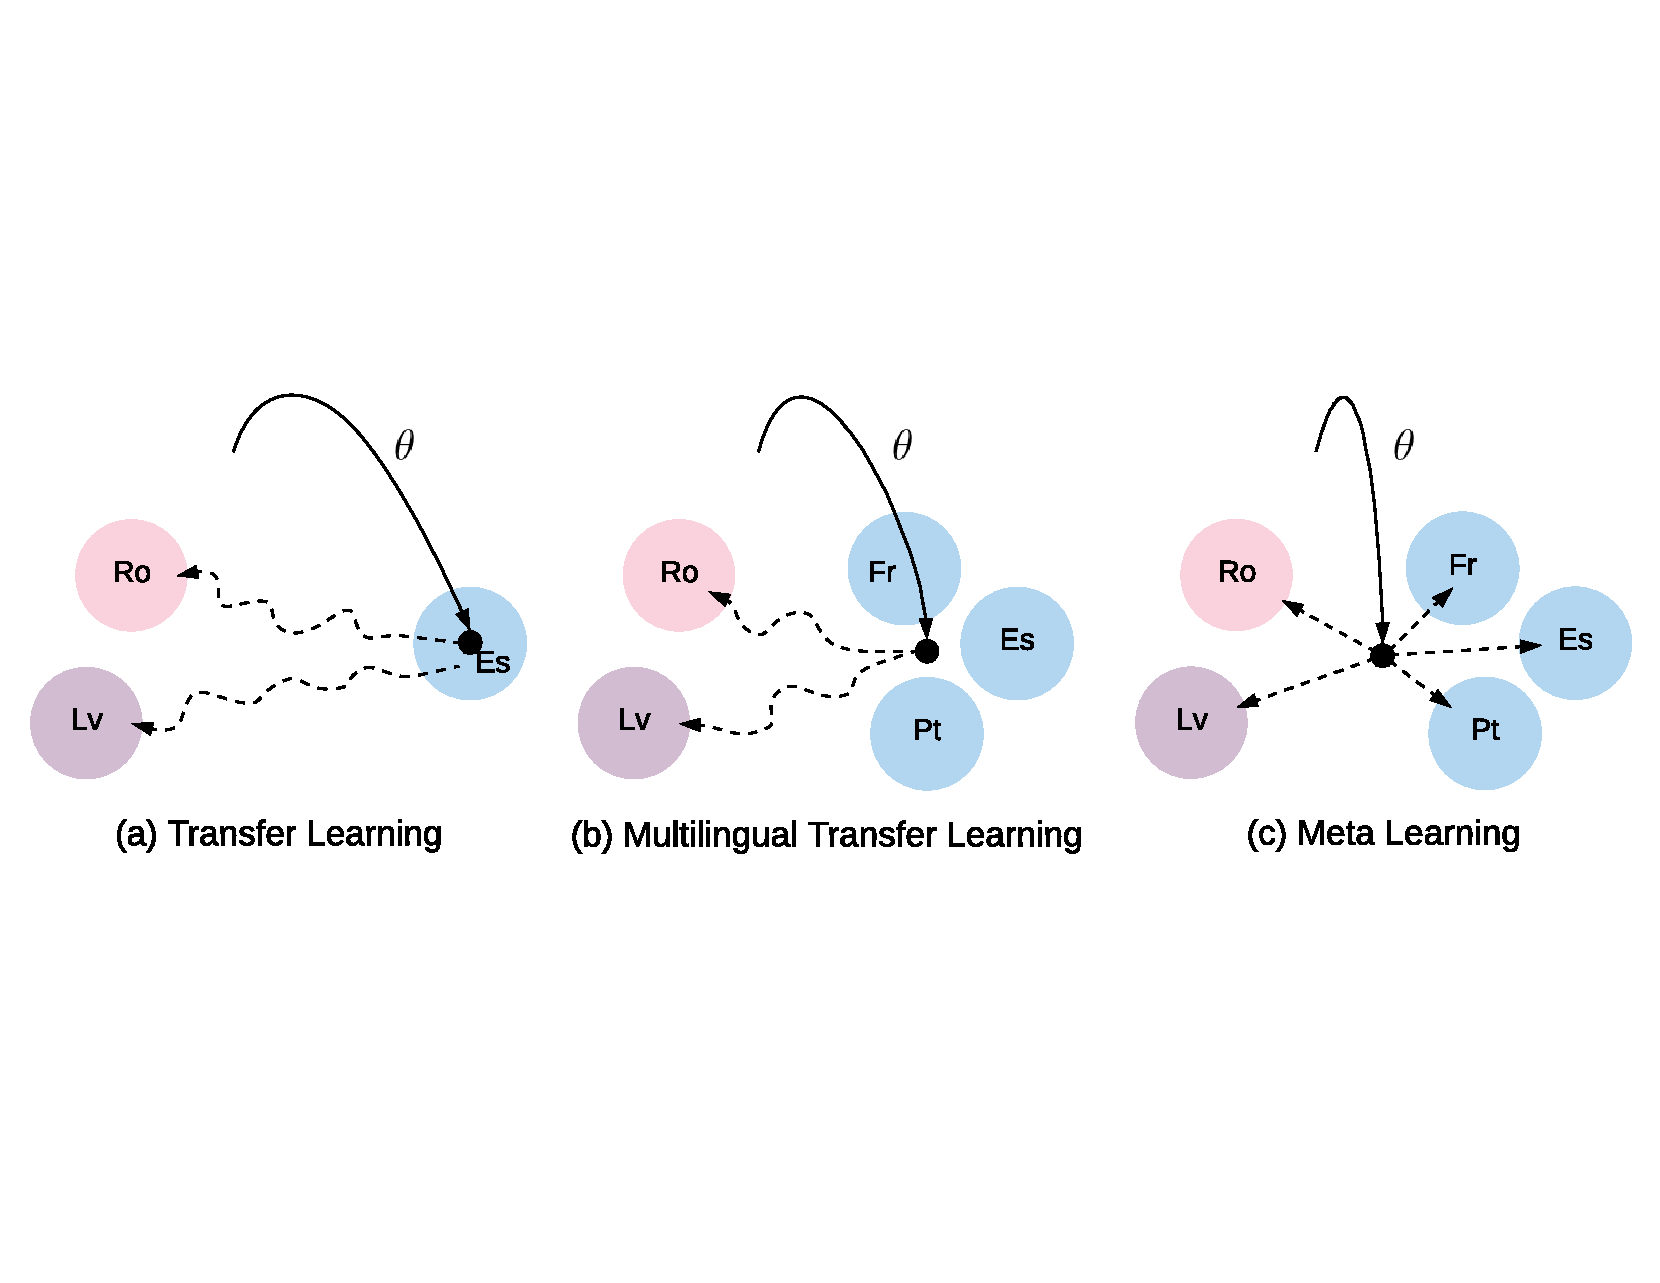
\includegraphics[width=\linewidth]{figs/meta/illust.pdf}%
}
%\vspace{-15pt}
\end{figure*}

In Fig.~\ref{cp6.fig.illustration}, we contrast transfer learning, multilingual learning and meta-learning using three source language pairs (Fr-En, Es-En and Pt-En) and two target pairs (Ro-En and Lv-En). Transfer learning trains an NMT system specifically for a source language pair (Es-En) and finetunes the system for each target language pair (Ro-En, Lv-En). Multilingual learning often trains a single NMT system that can handle many different language pairs (Fr-En, Pt-En, Es-En), which may or may not include the target pairs (Ro-En, Lv-En). If not, it finetunes the system for each target pair, similarly to transfer learning. Both of these however aim at directly solving the source tasks. On the other hand, meta-learning trains the NMT system to be {\it useful for fine-tuning} on various tasks including the source and target tasks. This is done by repeatedly simulating the learning process on low-resource languages using many high-resource language pairs (Fr-En, Pt-En, Es-En). 



% which has been proved very successful on low-resource neural machine translation. 

% The major difference is that, for multi-ligual transfer learning, the objective is to jointly optimize the likelihood across multiple languages with most of the parameters shared. The target low resource language can be either jointly training with other languages, or be fine-tuned after trained on high resource languages. Similar to Eq.~\ref{eq.meta} we have
% \begin{equation}
%     \label{eq.multi}
%     \max_{\theta} \sum_{k=1}^K \sum_{X, Y}^{\mathcal{T}^k} \log p(Y|X; \theta)
% \end{equation}
% where we do not have inner-loop updates. 

% TODO: Intert a discussion about Figure.2

\subsection{Unified Lexical Representation}% for MetaNMT}
\label{cp6.sec.ulr}

%\todo{KC: shorten this section. It's really difficult to shorten it.}

\paragraph{I/O mismatch across language pairs}
One major challenge that limits applying meta-learning for low resource machine translation is that
the approach outlined above assumes the input and output spaces are shared across all the source and target tasks. This, however, does not apply to machine translation in general due to the vocabulary mismatch across different languages. In multilingual translation, this issue has been tackled by using a vocabulary of sub-words~\citep{sennrich2015improving} or characters~\citep{lee2016fully} shared across multiple languages. This surface-level sharing is however limited, as it cannot be applied to languages exhibiting distinct orthography (e.g., Indo-Euroepan languages vs. Korean.) 

% One major challenge that limits applying MAML for NMT is that this learning algorithm implicitly assumes similar a I/O space at training and testing so that it can be adapted quickly with few examples. 
% %It is natural for tasks such as few-shot image classification where raw pixels are used as inputs. 
% However for NMT, each token from one language is firstly associated with an embedding vector $\epsilon[x]$ based on an unique token index $x$ before read by the following layers. $\epsilon$ is the embedding matrix which is trained jointly with $\theta$\footnote{For simplicity, we denote $\epsilon$ as the embedding, while $\theta$ as the rest of parameters of an NMT model.} from random initialization and typically differs across languages. 

% Therefore, although different languages share intrinsic similarities at both syntactic and semantic levels, the conventional MAML cannot learn good initialization for the embedding for fast adaptation.
% %the target language pairs might not even share the vocabularies with all other languages during training. 
% \alert{KC: the following is not an issue with the I/O space mismatch, but the issue of sparsity.}
% Furthermore, for translating very low resource languages (e.g., hundreds of training examples), a large proportion of tokens may never appear during adaptation, which is impossible to get meaningful translation for them.

\paragraph{Universal Lexical Representation (ULR)} 

We tackle this issue by dynamically building a vocabulary specific to each language using a key-value memory network~\citep{miller2016key,gulcehre2018dynamic}, which was introduced in detail in Chapter~\ref{ulr}, in \S\ref{cp5.sec.unilex} as the universal lexical representation (ULR) where we formulate the universal embedding for each word $x$ as a weighted sum of the embeddings $\epsilon_U$ of a set of universal tokens $u_1, ..., u_M$. Here we use the resulted universal embedding matrix for each word (as computed in Eq.~\eqref{cp5.eq.universal_embed}) as the initialized embedding $\epsilon^0[x]$ for each word of each input language.


%done successfully for low-resource machine translation recently by \citet{gu2018universal}. We start with multilingual word embedding matrices $\epsilon^k_{\text{query}} \in \mathbb{R}^{|V_k| \times d}$ pretrained on large monolingual corpora, where $V_k$ is the vocabulary of the $k$-th language. These embedding vectors can be obtained with small dictionaries of seed word pairs~\citep{artetxe2017learning,smith2017offline} or in a fully unsupervised manner~\citep{zhang2017earth,alexis2018word}. We take one of these languages $k'$ to build universal lexical representation consisting of a universal embedding matrix $\epsilon_u \in \mathbb{R}^{M \times d}$ and a corresponding
%% KC: $k$ is overloaded with too many semantics
%key matrix $\epsilon_{\text{key}} \in \mathbb{R}^{M \times d}$, where $M < |V_k'|$. Both $\epsilon^k_{\text{query}}$ and $\epsilon_{\text{key}}$ are fixed during meta-learning. We then compute the language-specific embedding of token $x$ from the language $k$ as the convex sum of the universal embedding vectors by
%\[
%\epsilon^0[x] = \sum_{i=1}^M \alpha_i \epsilon_u[i],
%\]
%where 
%$\alpha_i \propto \exp\left\{ -\tfrac{1}{\tau} \epsilon_{\text{key}}[i]^\top A \epsilon^k_{\text{query}} [x] \right\}$ and $\tau$ is set to $0.05$. This approach allows us to handle languages with different vocabularies using a fixed number of shared parameters ($\epsilon_u$, $\epsilon_{\text{key}}$ and $A$.) 

\paragraph{Learning of ULR}

It is not desirable to update the universal embedding matrix $\epsilon_U$ when fine-tuning on a small corpus which contains a limited set of unique tokens in the target language, as it could adversely influence the other tokens' embedding vectors. We thus estimate the change to each embedding vector induced by language-specific learning by a separate parameter $\Delta \epsilon^k[x]$:
\begin{equation}
	\epsilon^k[x] = \epsilon^0[x] + \Delta \epsilon^k[x].
\end{equation}
During language-specific learning, the ULR $\epsilon^0[x]$ is held constant, while only $\Delta \epsilon^k[x]$ is updated, starting from an all-zero vector. On the other hand, we hold $\Delta \epsilon^k[x]$'s constant while updating $\epsilon_U$ and $A$ during the meta-learning stage. 


% \alert{KC: TODO}

% Tackling on above challenges, it is essential to have a unified I/O space for MetaNMT. 
% For instance, considering the surface similarities (e.g. spelling, morphology, etc.), we can use a subword-based or character-based~\cite{lee2016fully} model to enforce all the languages share the same vocabularies. However, such surface-level sharing has limitations to apply to distinct languages (e.g. Indo-European languages and Korean). In practise, we also found that sharing sub-words fails when given extremely limited training data even for similar languages.

% Instead, we utilize a simple but effective method based on projected monolingual embedding which was recently proposed in \newcite{gu2018universal}. More precisely, we define a space for $M$ universal lexical tokens with the trainable embedding matrix $\epsilon_u\in\mathbb{R}^{M\times d}$. Thus, we can represent each input token $x$ from any language by querying with a distance measure $d(u_i,x)$:
% \begin{equation}
%  \label{eq.source word}
% \epsilon^0[x]=\sum_{i=1}^M\epsilon_u[u_i]\cdot \text{softmax}\left({-d(u_i,x)}/{\tau}\right),
% \end{equation}
% % where $q(u_i|x)$ is a conditional distribution in universal token space. $q(u_i|x)$ is computed by the distance metric:
% % \begin{equation}
% %  \label{eq.q distance}
% % q(u_i|x)=\frac{e^{\frac{d(u_i,x)}{\tau}}}{\sum_i e^{\frac{d(u_i,x)}{\tau}}},
% % \end{equation}
% where $\tau$ is the temperature. Following \newcite{gu2018universal}, one way to compute the distance is:
% %$d(u_i,x)$ measures the similarity between source word $x$ and universal token $u_i$ and it can be obtained by:
% \begin{equation}
%  \label{eq.d distance}
% d(u_i, x)=-\epsilon_k(u_i)\cdot A\cdot\epsilon_q(x)^\top,
% \end{equation}
% where $\epsilon_k$ are the \textit{key} vectors for universal tokens, and $\epsilon_q$ are the \textit{query} vectors for any specific input language. Both of the vectors are fixed can be easily obtained by learning embeddings from large monolingual corpora and then being projected to the same space based on a small dictionary\cite{smith2017offline} or in unsupervised~\cite{zhang2017earth,alexis2018word}. The transformation matrix $A$ initialized with identity matrix is learned in the training process.

% \paragraph{ULR as Initialized Word Embedding} 

% One major difference with \newcite{gu2018universal} is that in their work, the resulted universal vector (Eq.~\ref{eq.source word}) is jointly used with an individual embedding trained independently for each token. In contrast for meta learning, we assume each token only has one embedding $\epsilon[x]$ that is specially initialized by $\epsilon^0[x]$. It is equivalent to treat $\epsilon^0[x]$ as constant and learn an difference $\Delta\epsilon[x]$ in the inner-loop, while passing gradients from the updated vector $\Delta\epsilon[x] + \epsilon^0[x]$ to $\epsilon_u$ and $A$ in the outer-loop from Eq.~\ref{eq.source word} and \ref{eq.d distance}.


% \subsection{Unified I/O Space for MetaNMT}

% %\todo{KC: shorten this section. It's really difficult to shorten it.}

% \paragraph{Challenges}
% One major challenge that limits applying MAML for NMT is that the learning algorithm learns the network initialization for all the tasks, implicitly assuming similar a I/O space at training and testing so that it can be adapted quickly with few examples. %It is natural for tasks such as few-shot image classification where raw pixels are used as inputs. 
% However for NMT, each token from one language is firstly associated with an embedding vector $\epsilon[x]$ based on an unique token index $x$ before read by the following layers. $\epsilon$ is the embedding matrix which is trained jointly with $\theta$\footnote{For simplicity, we denote $\epsilon$ as the embedding, while $\theta$ as the rest of parameters of an NMT model.} from random initialization and typically differs across languages. 

% Therefore, although different languages share intrinsic similarities at both syntactic and semantic levels, the conventional MAML cannot learn good initialization for the embedding for fast adaptation.
% %the target language pairs might not even share the vocabularies with all other languages during training. 
% Furthermore, for translating very low resource languages (e.g., hundreds of training examples), a large proportion of tokens may never appear during adaptation, which is impossible to get meaningful translation for them.

% \paragraph{Universal Lexical Representation} Tackling on above challenges, it is essential to have a unified I/O space for MetaNMT. 
% For instance, considering the surface similarities (e.g. spelling, morphology, etc.), we can use a subword-based or character-based~\cite{lee2016fully} model to enforce all the languages share the same vocabularies. However, such surface-level sharing has limitations to apply to distinct languages (e.g. Indo-European languages and Korean). In practise, we also found that sharing sub-words fails when given extremely limited training data even for similar languages.

% Instead, we utilize a simple but effective method based on projected monolingual embedding which was recently proposed in \newcite{gu2018universal}. More precisely, we define a space for $M$ universal lexical tokens with the trainable embedding matrix $\epsilon_u\in\mathbb{R}^{M\times d}$. Thus, we can represent each input token $x$ from any language by querying with a distance measure $d(u_i,x)$:
% \begin{equation}
%  \label{eq.source word}
% \epsilon^0[x]=\sum_{i=1}^M\epsilon_u[u_i]\cdot \text{softmax}\left({-d(u_i,x)}/{\tau}\right),
% \end{equation}
% % where $q(u_i|x)$ is a conditional distribution in universal token space. $q(u_i|x)$ is computed by the distance metric:
% % \begin{equation}
% %  \label{eq.q distance}
% % q(u_i|x)=\frac{e^{\frac{d(u_i,x)}{\tau}}}{\sum_i e^{\frac{d(u_i,x)}{\tau}}},
% % \end{equation}
% where $\tau$ is the temperature. Following \newcite{gu2018universal}, one way to compute the distance is:
% %$d(u_i,x)$ measures the similarity between source word $x$ and universal token $u_i$ and it can be obtained by:
% \begin{equation}
%  \label{eq.d distance}
% d(u_i, x)=-\epsilon_k(u_i)\cdot A\cdot\epsilon_q(x)^\top,
% \end{equation}
% where $\epsilon_k$ are the \textit{key} vectors for universal tokens, and $\epsilon_q$ are the \textit{query} vectors for any specific input language. Both of the vectors are fixed can be easily obtained by learning embeddings from large monolingual corpora and then being projected to the same space based on a small dictionary\cite{smith2017offline} or in unsupervised~\cite{zhang2017earth,alexis2018word}. The transformation matrix $A$ initialized with identity matrix is learned in the training process.

% \paragraph{ULR as Initialized Word Embedding} One major difference with \newcite{gu2018universal} is that in their work, the resulted universal vector (Eq.~\ref{eq.source word}) is jointly used with an individual embedding trained independently for each token. In contrast for meta learning, we assume each token only has one embedding $\epsilon[x]$ that is specially initialized by $\epsilon^0[x]$. It is equivalent to treat $\epsilon^0[x]$ as constant and learn an difference $\Delta\epsilon[x]$ in the inner-loop, while passing gradients from the updated vector $\Delta\epsilon[x] + \epsilon^0[x]$ to $\epsilon_u$ and $A$ in the outer-loop from Eq.~\ref{eq.source word} and \ref{eq.d distance}.
% \subsection{Meta-Learning for Semi-Supervised Low Resource Translation}
% Not sure if it will work or not yet


% The overall algorithm can be seen as follows:
% \begin{algorithm}[H]
% \caption{Learning for Meta-NMT (placeholder as long as possible)}
% \label{algo1}
% \begin{algorithmic}[1]
% \small
% \Require{MT model ${\theta}$.}
% \State Initialize 
% \While{stopping criterion is not met}
% \For{$k=1...K$}  
% \State Let $Y'_k = \{y'_1, ..., y'_{T'}\}, X'_k = \{x'_1, ..., x'_{T'_s}\}$
% \For{$\tau=1...T'$}
% \State Generate key $c'_\tau = f_{\text{att}}(y'_{<\tau}, X'_k)$
% \EndFor 
% \EndFor
% \State Update $\phi \leftarrow \phi  +\gamma\frac{\partial}{\partial \phi} \sum_{t=1}^T\log p(y_t|\cdot)$
% \EndWhile
% \end{algorithmic}
% \end{algorithm}


\section{Experiments}
\label{cp6.sec.exps}

%We extensively study the effectiveness of the proposed MetaNMT for fast parameter adaptation of NMT given limited training examples. We evaluated the algorithm on four simulated low resource language pairs with variant auxiliary languages used for meta-training. Both random initialization and multilingual training are used as baselines.

\subsection{Dataset}

%\paragraph{Dataset} We empirically evaluate the proposed \textsc{ZR-NMT} on $4$ languages -- Romanian (Ro) / Latvian (LV) / Korean (KO) / Levantine Arabic (LEV)\footnote{A spoken dialect of standard Arabic.} -- translating to English (En) in near zero-resource settings. To achieve this, single or multiple auxiliary languages from Czech (Cs), German (De), Greek (El), Spanish (Es), Finnish (Fi), French (Fr),  Italian (It), Portuguese (Pt), Russian (Ru) and Modern Standard Arabic (MSA) are jointly trained to translate to English.

\paragraph{Target Tasks}
We show the effectiveness of the proposed meta-learning method for low resource NMT with extremely limited training examples on five diverse target languages: Romanian (Ro) from WMT'16,\footnote{
\url{http://www.statmt.org/wmt16/translation-task.html}
}
Latvian (Lv), Finnish (Fi), Turkish (Tr) from WMT'17,\footnote{
\url{http://www.statmt.org/wmt17/translation-task.html}
}
and Korean (Ko) from Korean Parallel Dataset.\footnote{
\url{https://sites.google.com/site/koreanparalleldata/}
}
We use the officially provided train, dev and test splits for all these languages. %\alert{how do we split Ko?}
The statistics of these languages are presented in Table~\ref{cp6.table.full-dataset}. We simulate the low-resource translation scenarios by randomly sub-sampling the training set with different sizes.

\begin{table}[hptb]
\centering
%\resizebox{\textwidth}{!}{
\begin{tabular}{rcc|rr}
\toprule
%  &\multicolumn{2}{c}{Bleu score}&\multicolumn{2}{c}{Bleu score}\\
& \# of sents. & \# of En tokens & Dev & Test\\
\midrule
Ro-En&$0.61$ M &$16.66$ M&$-$&$31.76$  \\
Lv-En&$4.46$ M &$67.24$ M&$20.24$&$15.15$\\
Fi-En&$2.63$ M &$64.50$ M&$17.38$&$20.20$  \\
Tr-En&$0.21$ M & \ \ $5.58$ M &$15.45$&$13.74$ \\
Ko-En&$0.09$ M & \ \ $2.33$ M &$6.88$&$5.97$ \\
\bottomrule
\end{tabular}
%}
\caption{Statistics of full datasets of the target language pairs. BLEU scores on the dev and test sets are reported from a supervised Transformer model with the same architecture.}
\label{cp6.table.full-dataset}
\end{table}



\paragraph{Source Tasks}

We use the following languages from Europarl\footnote{
\url{http://www.statmt.org/europarl/}
}:
Bulgarian (Bg),
Czech (Cs), 
Danish (Da),
German (De),
Greek  (El),
Spanish (Es),
Estonian  (Et),
French (Fr),
Hungarian   (Hu),
Italian (It),
Lithuanian  (Lt),
Dutch   (Nl),
Polish  (Pl),
Portuguese  (Pt),
Slovak  (Sk),
Slovene (Sl) and
Swedish (Sv), in addition to Russian (Ru)\footnote{
A subsample of approximately 2M pairs from WMT'17.
} to learn the intilization for fine-tuning. In our experiments, different combinations of source tasks are explored to see the effects from the source tasks.

% We employ $18$ languages as source tasks during meta-train, which includes all languages from Europarl\footnote{http://www.statmt.org/europarl/} except for those used as target tasks, i.e., 
% Bulgarian (Bg),
% Czech (Cs), 
% Danish (Da),
% German (De),
% Greek  (El),
% Spanish (Es),
% Estonian  (Et),
% French (Fr),
% Hungarian   (Hu),
% Italian (It),
% Lithuanian  (Lt),
% Dutch   (Nl),
% Polish  (Pl),
% Portuguese  (Pt),
% Slovak  (Sk),
% Slovene (Sl),
% Swedish (Sv). In addition, a subset ($\sim 2$ M sentence pairs) of Russian (Ru) from WMT'17 is also incorporated. In our experiments, different combinations of source tasks are explored to see the effects take from the source tasks.



\paragraph{Validation}

We pick either Ro-En or Lv-En as a validation set for meta-learning and test the generalization capability on the remaining target tasks. This allows us to study the strict form of meta-learning, in which target tasks are unknown during both training and model selection.




% 

% Ro and Lv are selected to be the meta-validation sets which are utilized to track the progress of the meta-model. Under this setting, we can carefully investigate the generalization capability of the proposed meta-learning approach. 

% By default, we only consider $\rightarrow\!\text{En}$ tasks. 
% We consider $4$ diverse languages as the main target tasks, including Romanian (Ro) from WMT'16\footnote{http://www.statmt.org/wmt16/translation-task.html}, Latvian (Lv), Finnish (Fi) and Turkish (Tr) from WMT'17\footnote{http://www.statmt.org/wmt17/translation-task.html} with official train, dev and test datasets. For an optional comparison with very distant languages, we also investigate using Korean (Ko)\footnote{https://sites.google.com/site/koreanparalleldata/} as the exceptional target language. The detailed statistics of the target tasks are shown in Table.~/ref{table:full dataset}, some of which are low resource-enough already. 
% In our experiments, random sampling are further performed to simulate extremely low resource settings from which we test the effectiveness of the proposed method. 


\paragraph{Preprocessing and ULR Initialization}

As described in \textsection\ref{cp6.sec.ulr}, we initialize the query embedding vectors $\epsilon_{K}^k$ of all the languages. For each language, we use the monolingual corpora built from Wikipedia\footnote{
We use the most recent Wikipedia dump (2018.5) from \url{https://dumps.wikimedia.org/backup-index.html}. 
}
and the parallel corpus. The concatenated corpus is first tokenized and segmented using byte-pair encoding~\citep[BPE,][]{sennrich2016edinburgh}, resulting in $40,000$ subwords for each language. We then estimate word vectors using fastText~\citep{bojanowski2016enriching}. Different from the method proposed in Chapter~\ref{ulr} where we used a short-list of seed words to align the embeddings, we align the pre-trained word embeddings across all the languages in an unsupervised way using MUSE~\citep{alexis2018word} to get multilingual word vectors. We use the multilingual word vectors of the 20,000 most frequent words in English to form the universal embedding matrix $\epsilon_U$. 
% Following \citet{gu2018universal}, tokens of all other languages are attached with special language tags.



% We empirically evaluate the proposed Universal NMT system on $3$ languages -- Romanian (Ro) / Latvian (Lv) / Korean (Ko)  -- translating to English (En) in near zero-resource settings. To achieve this, single or multiple auxiliary languages from Czech (Cs), German (De), Greek (El), Spanish (Es), Finnish (Fi), French (Fr),  Italian (It), Portuguese (Pt) and Russian (Ru) are jointly trained. The detailed statistics and sources of the available parallel resource can be found in Table~\ref{table.data}, where we further down-sample the corpora for the targeted languages to simulate zero-resource. 
% As the origin of this work, we use the most recent wikidump\footnote{https://dumps.wikimedia.org/backup-index.html} as our monolingual data for training monolingual embeddings considering it covers all the languages we need and shares the same domains across languages.
% We tokenize and segment all monolingual and parallel data using byte-pair encoding \citep[BPE,][]{sennrich2016edinburgh}. $40,000$ BPE operations are applied for each language independently. We use fastText~\cite{bojanowski2016enriching}\footnote{https://github.com/facebookresearch/fastText} to learn the monolingual embedding from both the monolingual and parallel data, and apply MUSE~\cite{alexis2018word}\footnote{https://github.com/facebookresearch/MUSE} to get aligned word embeddings into the same space. As we are considering meta-learning for translation of very low resource languages, the unsupervised embeddings with  adversarial training and iterative refinement are used. Following \newcite{gu2018universal}, we use the top $20,000$ most frequent English words as the universal tokens to query from. Tokens of all other languages are attached with special language tags. 




%which were selected to be similar to Romanian. The second set consists of all the languages in the first set as well as Russian (Ru) and Czech (Cz), which were included because of their similarity to Latvian. 

\subsection{Model and Learning}

\paragraph{Model} 

We utilize the recently proposed Transformer \citep{vaswani2017attention} as an underlying NMT system (which is also different and better than the previous chapter). We implement Transformer in this paper based on \citep{Gu2017NonAutoregressiveNM}\footnote{
    \url{https://github.com/salesforce/nonauto-nmt}
}
and modify it to use the universal lexical representation from \textsection\ref{cp6.sec.ulr}. We use the default set of hyperparameters ($d_\text{model} = d_{\text{hidden}} = 512$, $n_\text{layer}=6$, $n_\text{head}=8$, $n_\text{batch}=4000$, $t_\text{warmup} = 16000$) for all the language pairs and across all the experimental settings. We refer the readers to \citep{vaswani2017attention,Gu2017NonAutoregressiveNM} for the details of the model. However, since the proposed meta-learning method is model-agnostic, it can be easily extended to any other NMT architectures, e.g. RNN-based sequence-to-sequence models with attention~\citep{bahdanau2014neural}.


% We leverage Transformer \cite{vaswani2017attention} -- a recently proposed state-of-the-art architecture --  as the base model to perform all the experiments. 
% More precisely, the Transformer model consists of an encoder stack and a decoder stack. The encoder is composed of a stack of identical blocks where each block contains two sub-layers: a multi-head self-attention layer and a position-wise fully connected feed-forward network. The decoder also consists of identical blocks, where for each block the decoder adds a multi-head attention over the output of the encoder stack. 
% The last layer of the decoder outputs translation in auto-regressively.

% We implemented the Transformer model using PyTorch based on the released code used in~\newcite{Gu2017NonAutoregressiveNM}\footnote{https://github.com/salesforce/nonauto-nmt}, where we modify their model to enable emebddings to be initialized by the universal lexical representation for any input languages.
% We use a default set of hyper-parameters ($d_\text{model} = d_{\text{hidden}} = 512$, $n_\text{layer}=6$, $n_\text{head}=8$, $n_\text{batch}=4000$, $t_\text{warmup} = 16000$) for all the language pairs for both \textit{learn} and \textit{meat-learn} stages.




\paragraph{Learning}
We meta-learn using various sets of source languages to investigate the effect of source task choice. For each episode, by default, we use a single gradient step of language-specific learning with Adam~\citep{kingma2014adam} per computing the meta-gradient, which is computed by the first-order approximation in Eq.~\eqref{cp6.eq.meta-grad-first}. 

For each target task, we sample training examples to form a low-resource task. We build tasks of 4k, 16k, 40k and 160k English tokens for each language. We randomly sample the training set five times for each experiment and report the average score and its standard deviation. Each fine-tuning is done on a training set, early-stopped on a validation set and evaluated on a test set. In default without notation, datasets of 16k tokens are used.







% \alert{TODO: For the rest of experiments, I am using first order approx, 1 step Adam in the inner loop, and 0.2 x cross lingual objective.}

\paragraph{Fine-tuning Strategies}

The transformer consists of three modules; embedding, encoder and decoder. We update all three modules during meta-learning, but during fine-tuning, we can selectively tune only a subset of these modules. Following \citep{zoph2016transfer}, we consider three fine-tuning strategies; (1) fine-tuning all the modules (all), (2) fine-tuning the embedding and encoder, but freezing the parameters of the decoder (emb+enc) and (3) fine-tuning the embedding only (emb). %\alert{KC: change the plots accordingly.} 



% To extensively study the effectiveness and the generalization ability of the proposed metaNMT, we first \textit{meta-learn} different models with variant combinations of source language pairs. In default, we run one gradient step for the inner loop, and use the first order approximation to compute the meta-gradients. Experiments with more detailed ablation study are shown in the next section.
% Multilingual NMT baselines~\cite{gu2018universal} are also trained with the same data for comparison.

% For each target task, we sample sentences from the full datasets for the fast adaptation, forming training sets with $4$K, $16$K, $40$K, $160$K English tokens, each of which are repeated $5$ times. Considering we use a batch size of $4000$ tokens for all experiments, a sampled $4$K dataset fits one batch for training. For every run, a best model is selected based on the dev set, and then evaluated on the test set. The final scores are averaged over $5$ runs.






\subsection{Results}

% \subsection{Main Results}
\begin{figure*}[t]
\centering                      
\subfigure[Ro-En]{                   
\begin{minipage}[t]{0.48\linewidth}
\centering                                                         
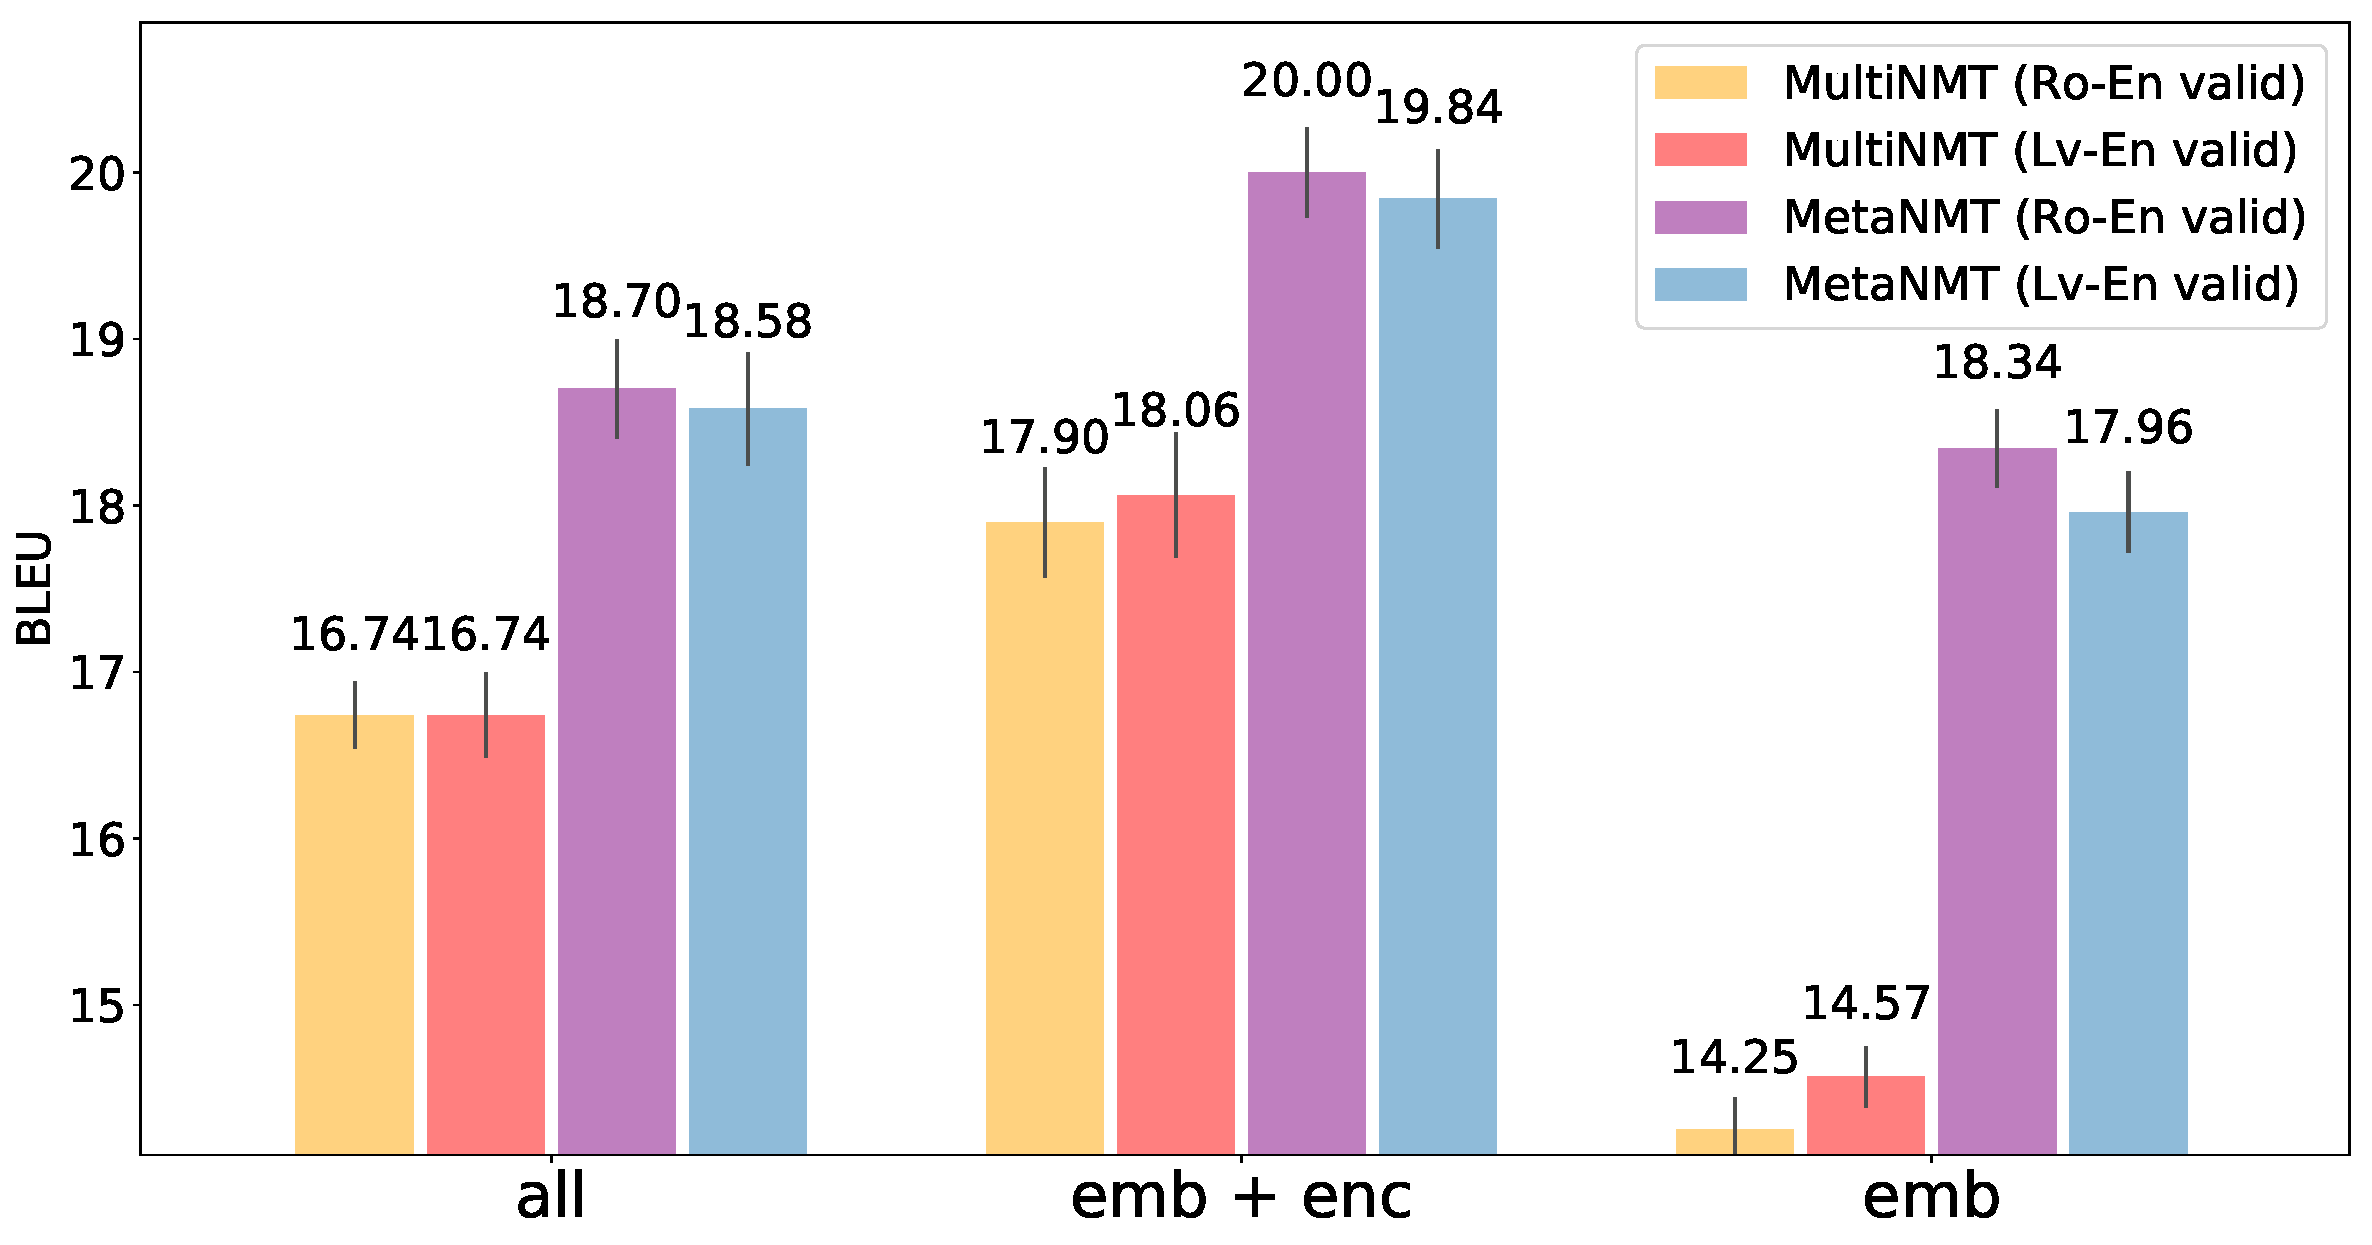
\includegraphics[width=\linewidth]{figs/meta/ro-en.pdf}              
\end{minipage}}
\subfigure[Lv-En]{                   
\begin{minipage}[t]{0.48\linewidth}
\centering                                                          
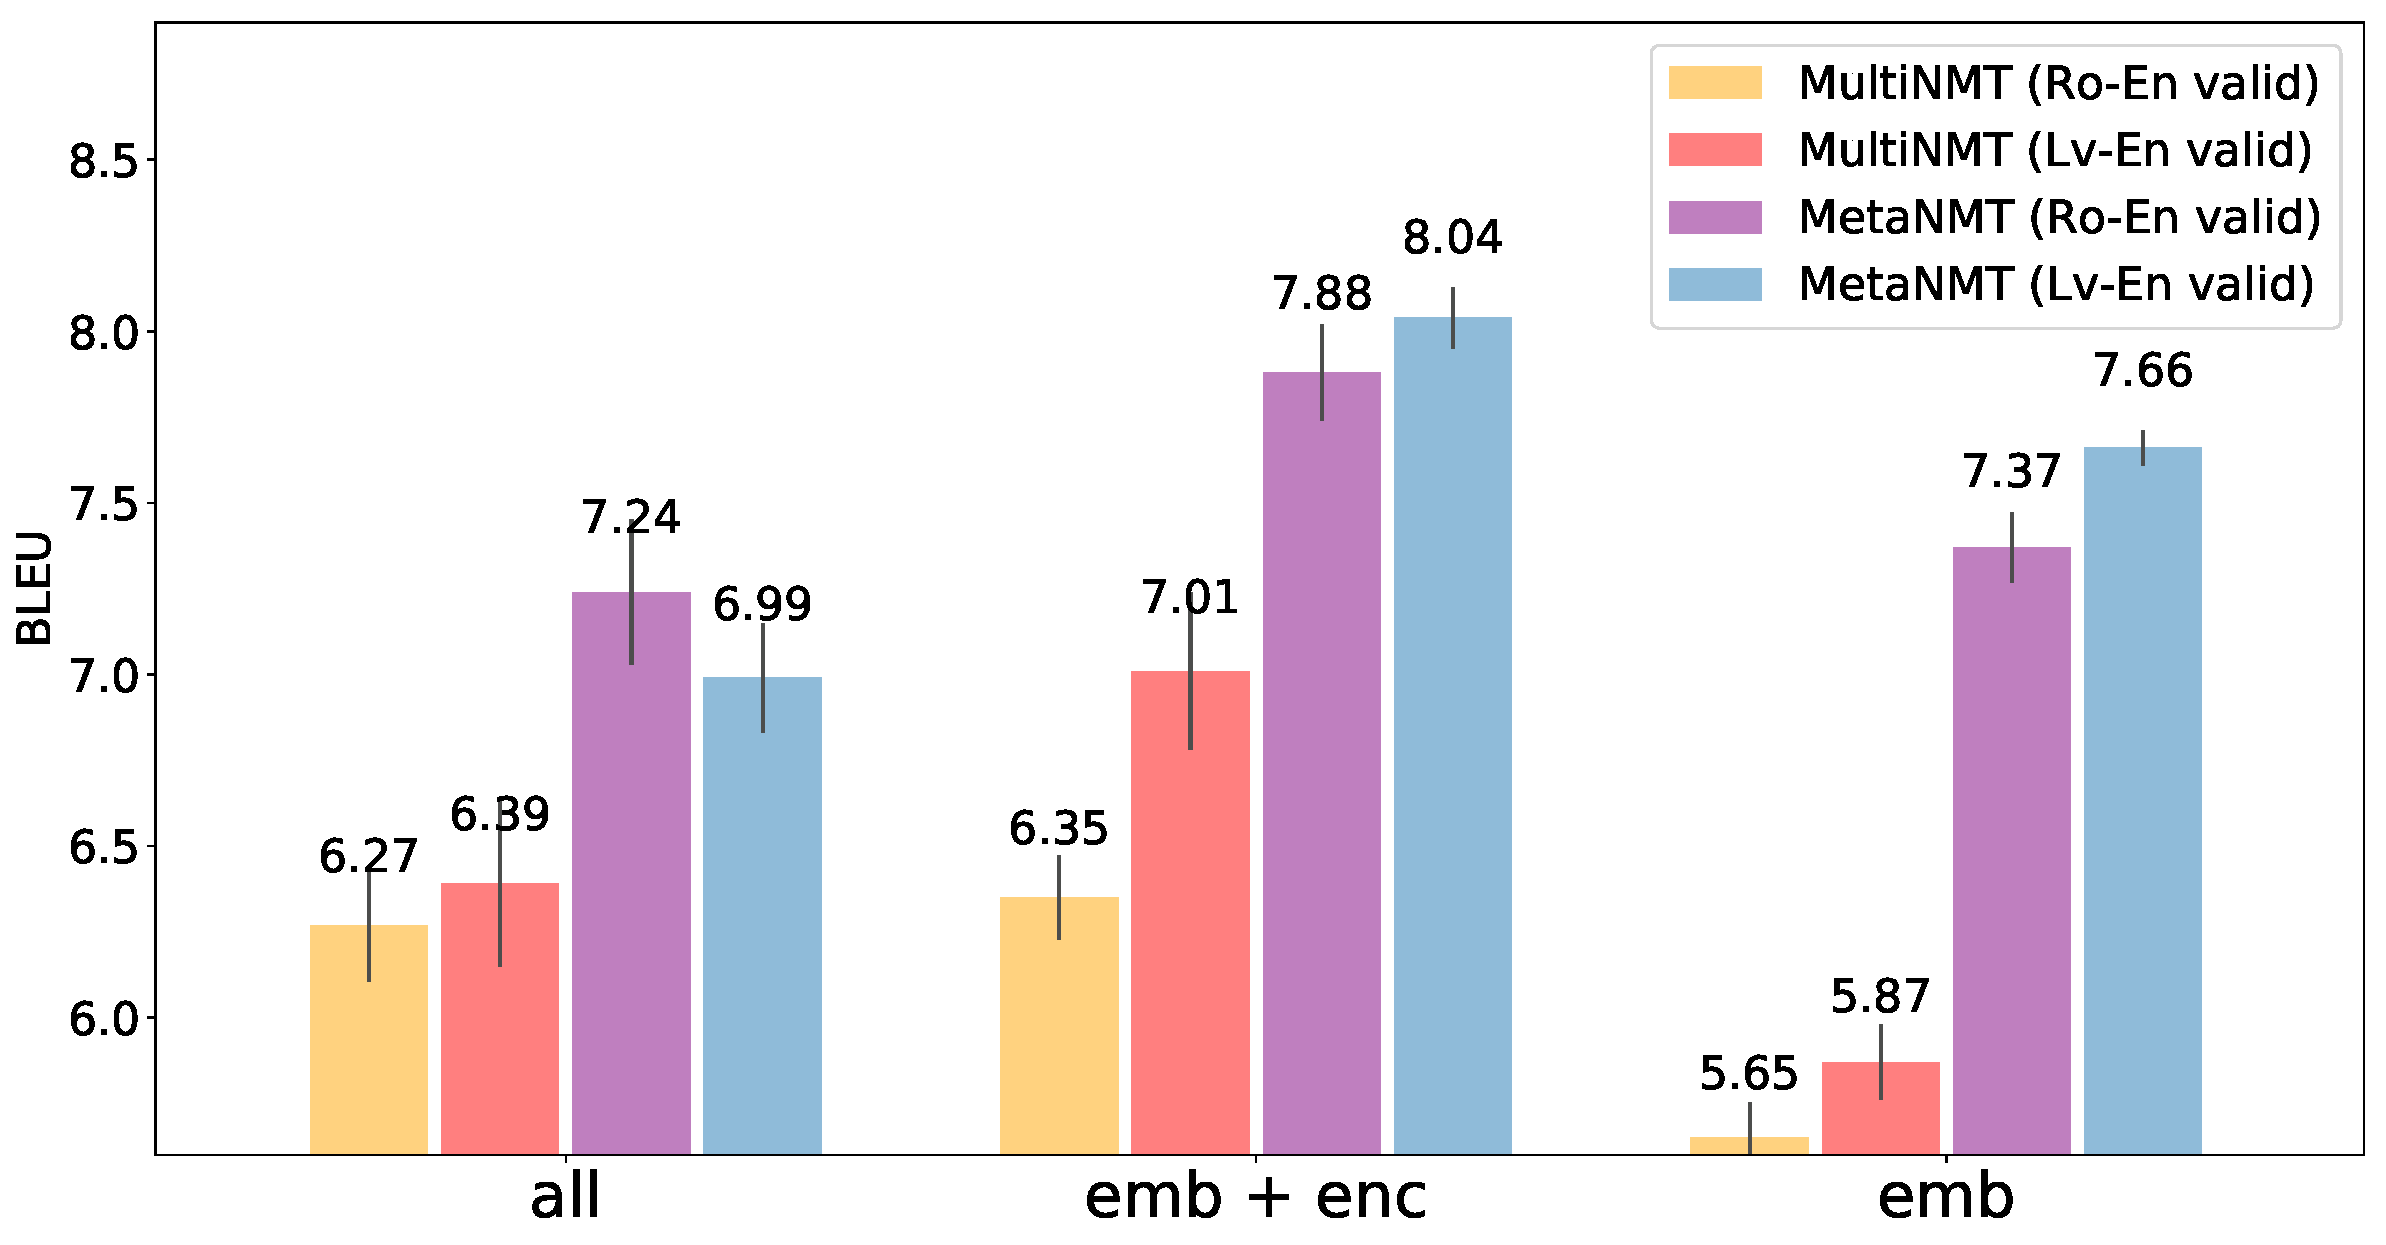
\includegraphics[width=\linewidth]{figs/meta/lv-en.pdf}                
\end{minipage}}
\subfigure[Fi-En]{                   
\begin{minipage}[t]{0.48\linewidth}
\centering                                                         
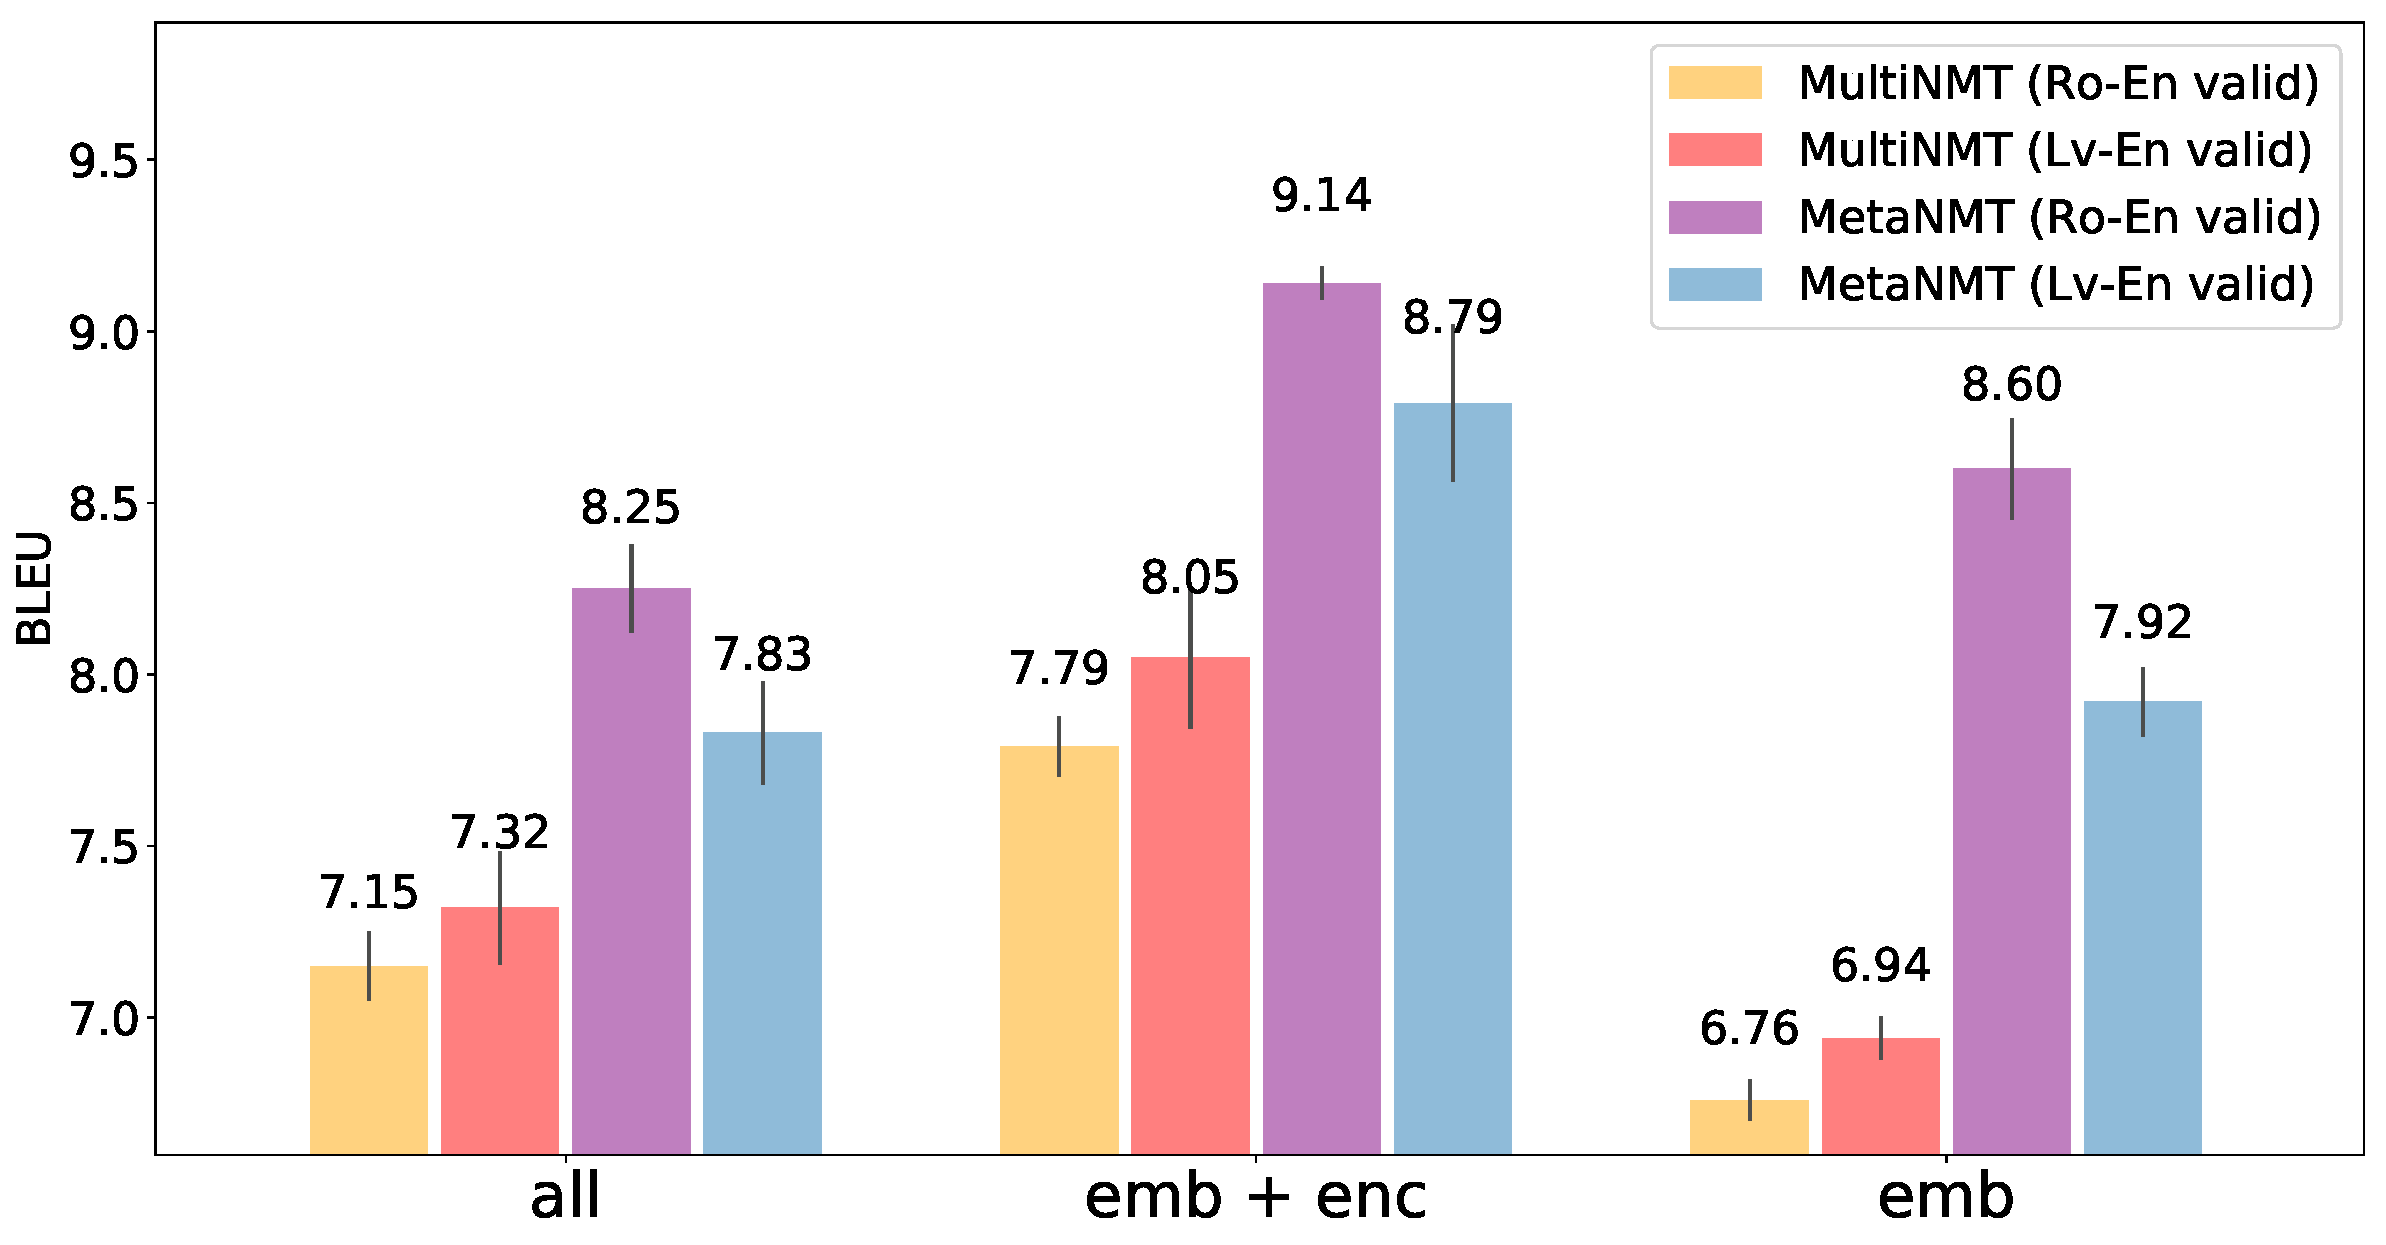
\includegraphics[width=\linewidth]{figs/meta/fi-en.pdf}              
\end{minipage}}
\subfigure[Tr-En]{                   
\begin{minipage}[t]{0.48\linewidth}
\centering                                                          
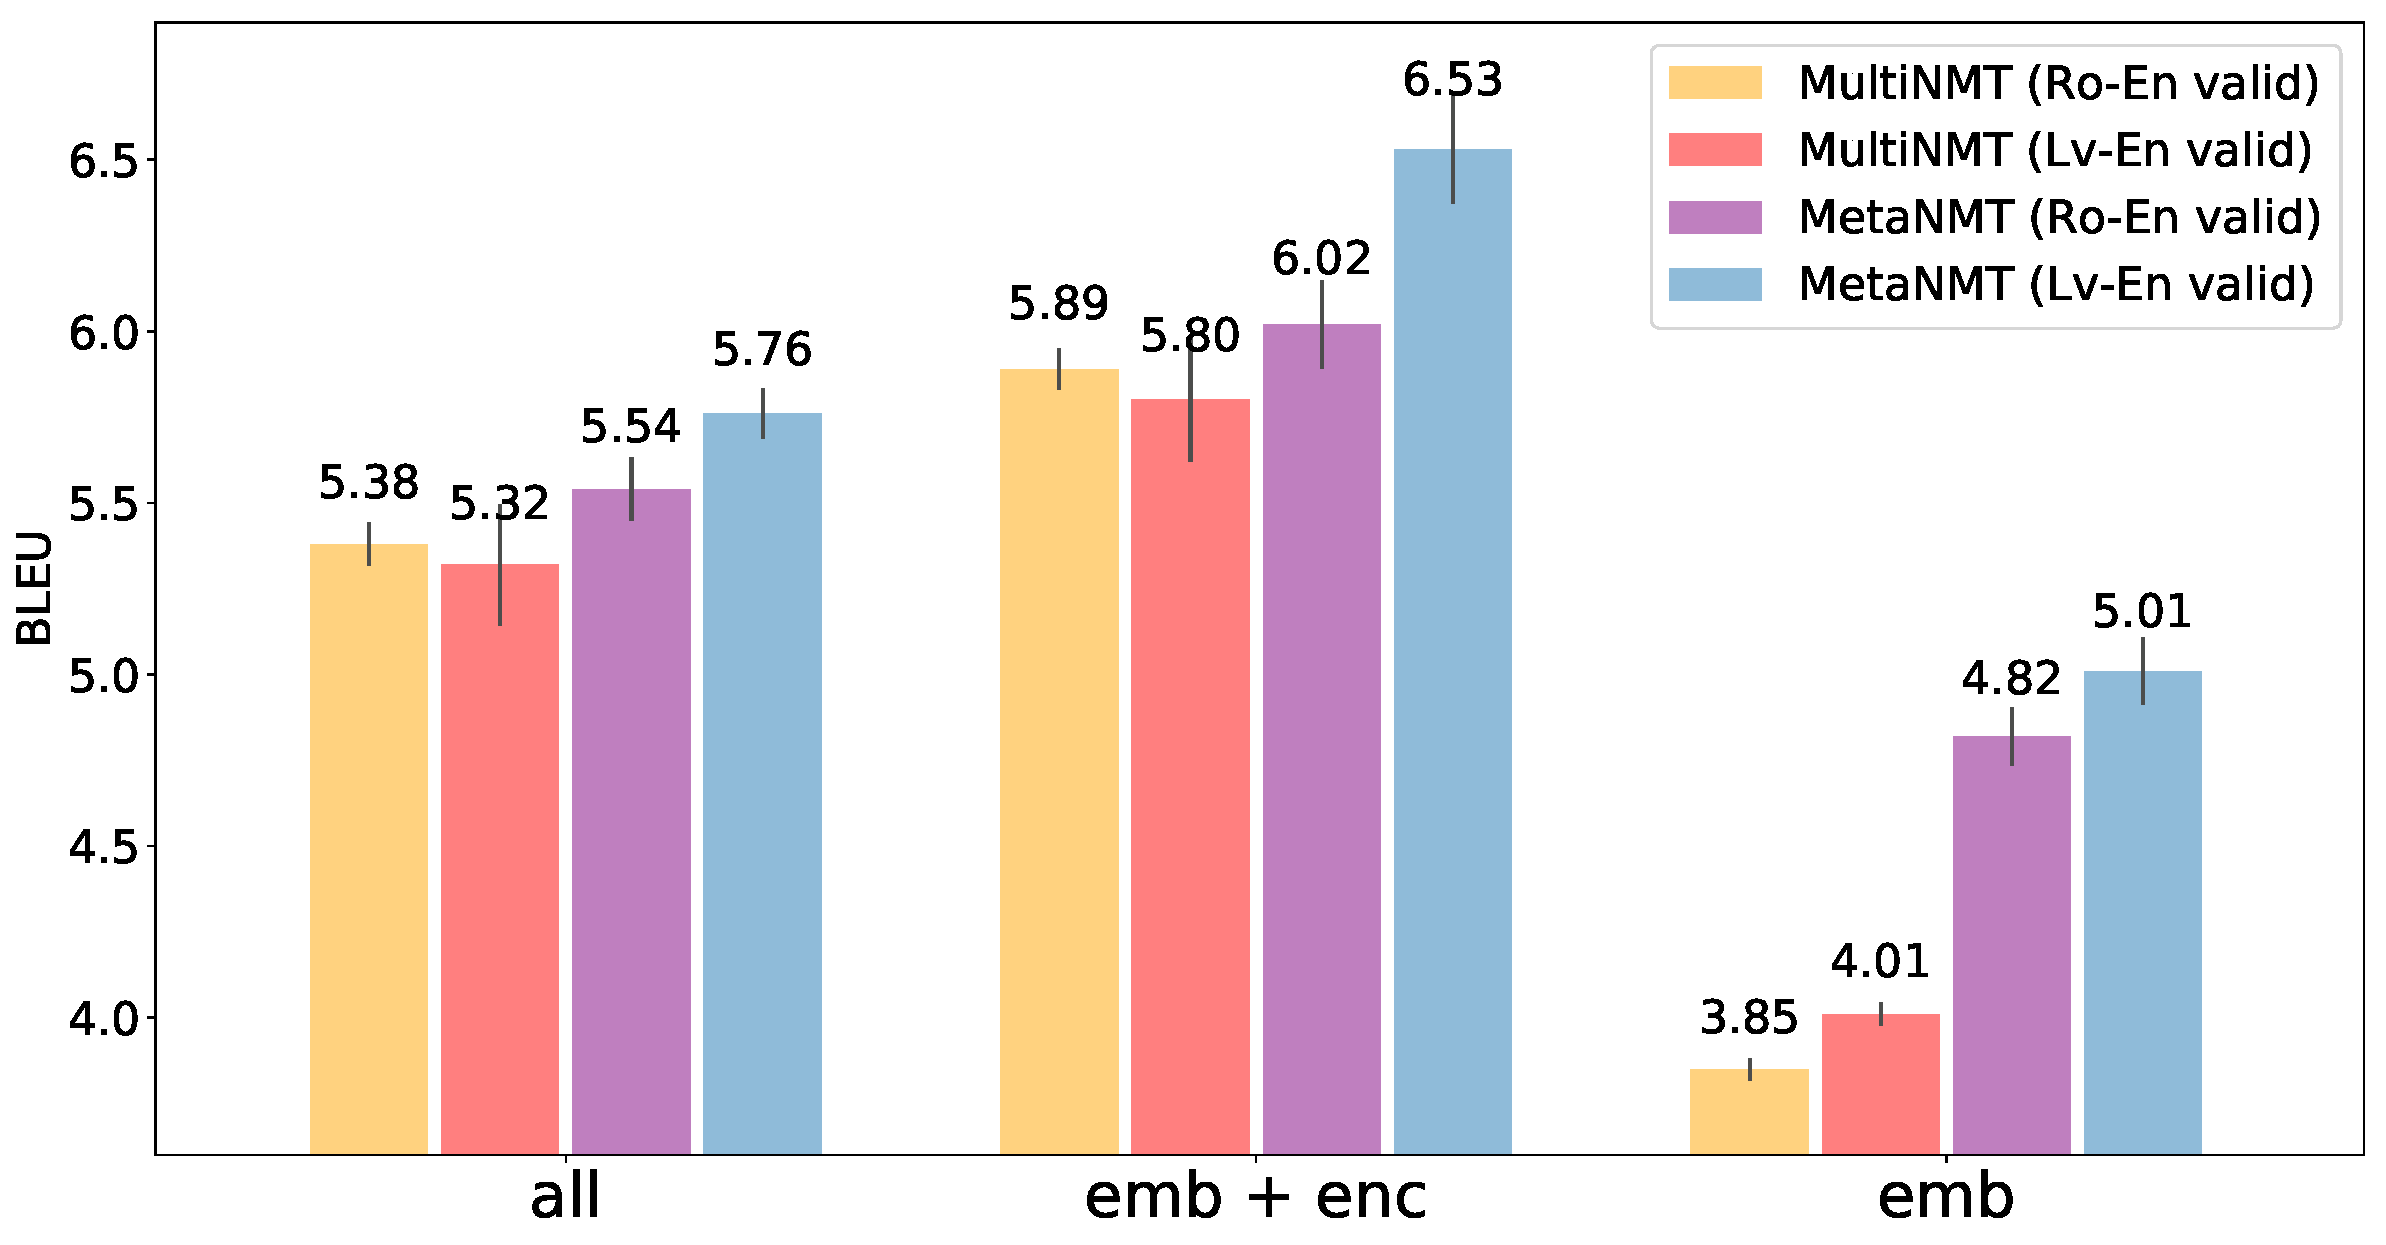
\includegraphics[width=\linewidth]{figs/meta/tr-en.pdf}                
\end{minipage}}
\caption{BLEU scores reported on test sets for \{Ro, Lv, Fi, Tr\} to En, where each model is first learned from 6 source tasks (Es, Fr, It, Pt, De, Ru) and then fine-tuned on randomly sampled training sets with around 16,000 English tokens per run. The error bars show the standard deviation calculated from 5 runs.} 
\label{cp6.fig.compare}                                                   
\end{figure*}

\paragraph{vs. Multilingual Transfer Learning}

We meta-learn the initial models on all the source tasks using either Ro-En or Lv-En as a validation task. We also train the initial models to be multilingual translation systems. We fine-tune them using the four target tasks (Ro-En, Lv-En, Fi-En and Tr-En; 16k tokens each) and compare the proposed meta-learning strategy and the multilingual, transfer learning strategy. As presented in Fig.~\ref{cp6.fig.compare}, the proposed learning approach significantly outperforms the multilingual, transfer learning strategy across all the target tasks regardless of which target task was used for early stopping. We also notice that the emb+enc strategy is most effective for both meta-learning and transfer learning approaches. With the proposed meta-learning and emb+enc fine-tuning, the final NMT systems trained using only a fraction of all available training examples achieve 2/3 (Ro-En) and 1/2 (Lv-En, Fi-En and Tr-En) of the BLEU score achieved by the models trained with full training sets.

\paragraph{Impact of Validation Tasks}

Similarly to training any other neural network, meta-learning still requires early-stopping to avoid overfitting to a specific set of source tasks. In doing so, we observe that the choice of a validation task has non-negligible impact on the final performance. For instance, as shown in Fig.~\ref{cp6.fig.compare}, Fi-En benefits more when Ro-En is used for validation, while the opposite happens with Tr-En. The relationship between the task similarity and the impact of a validation task must be investigated further in the future.
\begin{figure}[hptb]
    \centering
    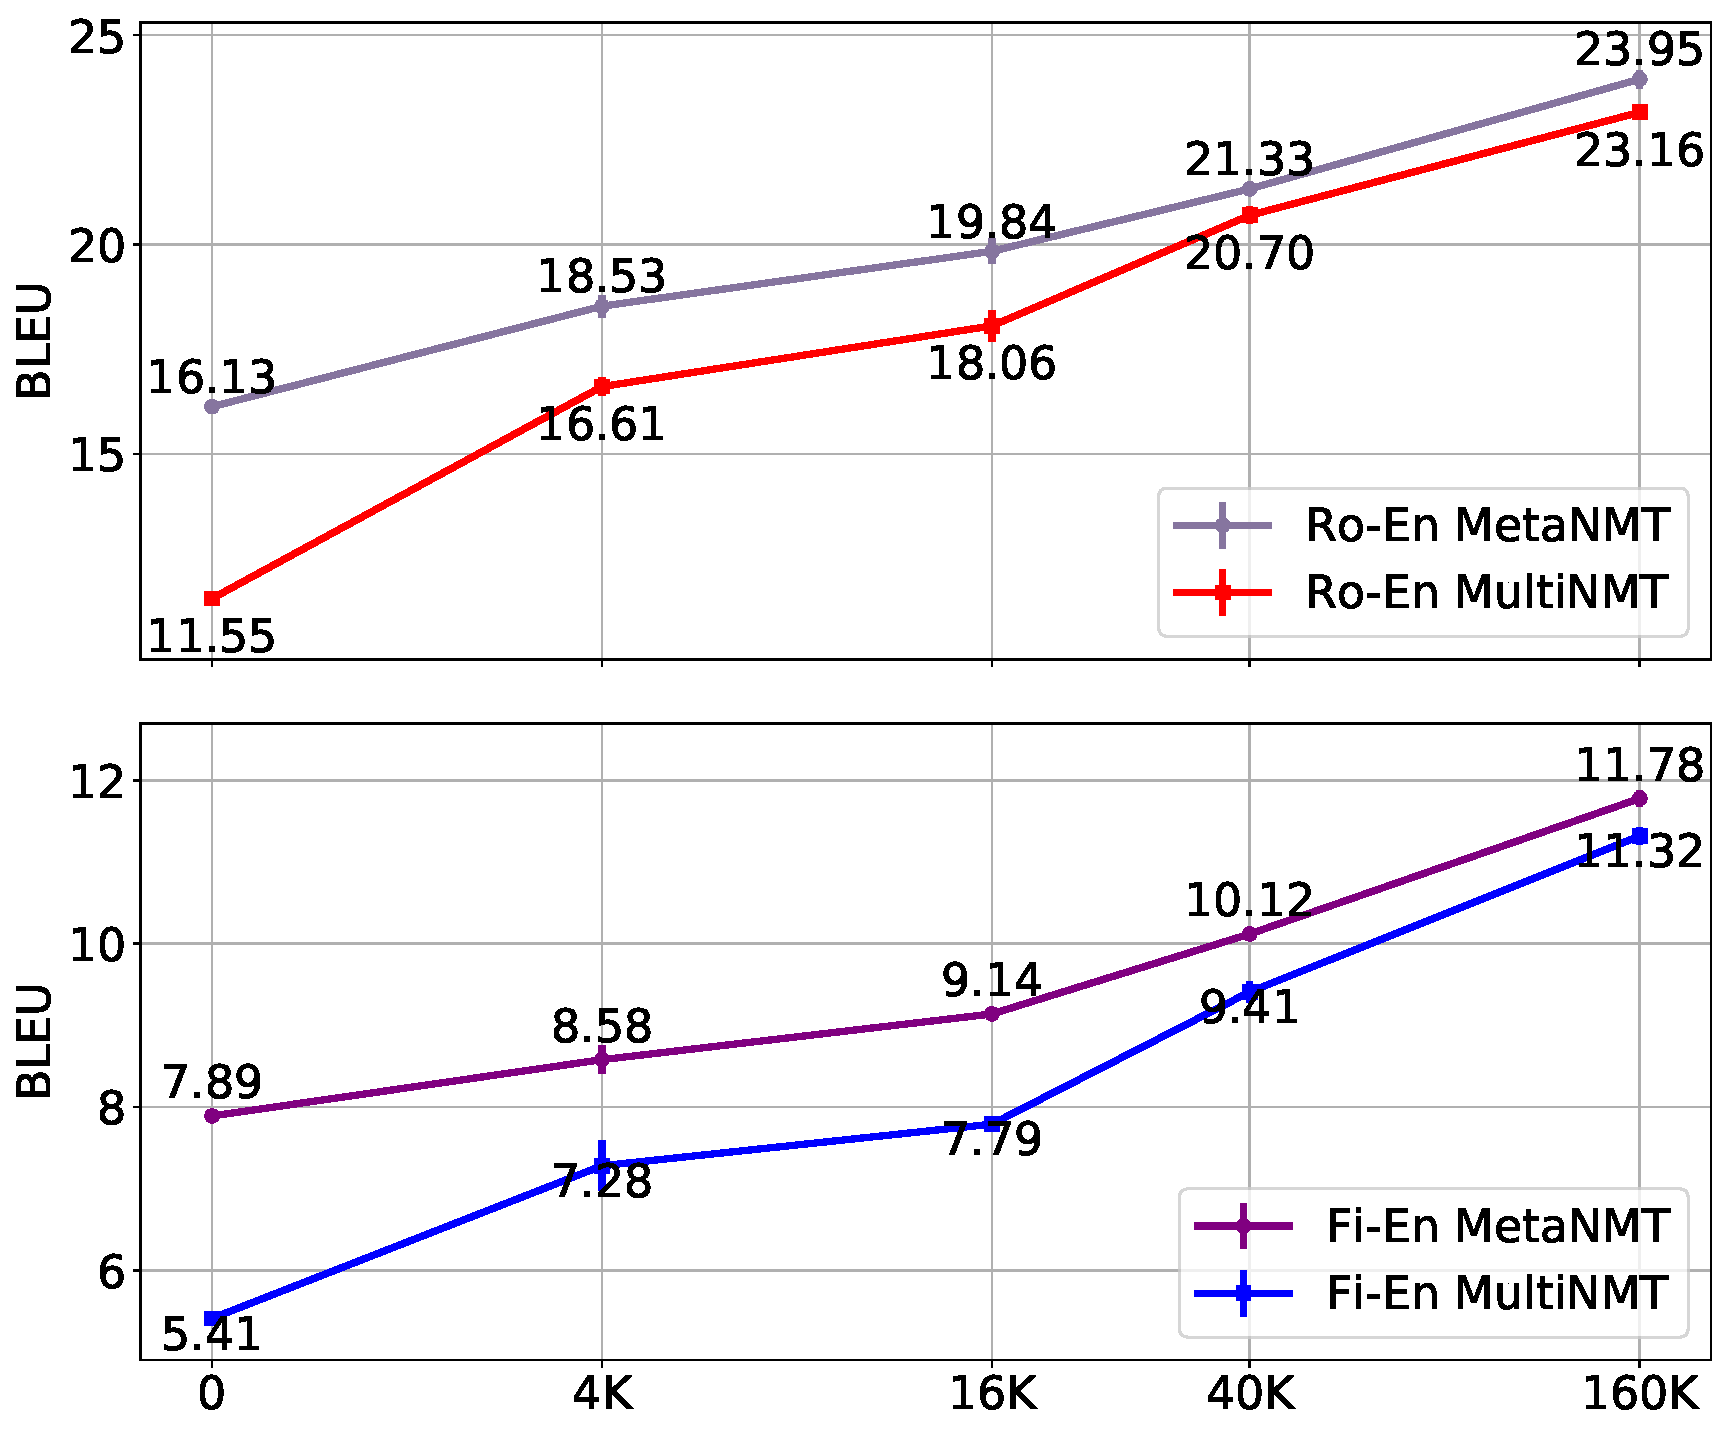
\includegraphics[width=0.8\linewidth]{figs/meta/support_size.pdf}
    \caption{BLEU Scores w.r.t. the size of the target task's training set.}
    \label{cp6.fig.support}
\end{figure}

% we also investigate the influence of using different languages as the validation task. 
% In general, 
% choosing the validation languages does have bias to the final performance on some target tasks, especially for the validation language itself and languages shares some similarities. For instance, the resulting BLEU scores of Fi-En with Ro as the validation task are higher in all the fine-tuning strategies of MetaNMT. In contrast, the performance on Tr-En does the opposite.

% Firstly, for training, choosing Lv-En as validation set benefits its performance other than a little drop of Tr-En in all and emb+enc finetune-tuning strategies. 
% For MetaNMT, its performance of choosing Ro-En as validation set is better than that of choosing Lv-En for Ro-En and Fi-En. However, Lv-En and Tr-En have the opposite results. 
% Secondly, we can see that the improvements of using different validation sets are different evidently. For Ro-En, Lv-En and Fi-En, the improvements of choosing Ro-En from MultiNMT to MetaNMT as validation set are greater than that of choosing Lv-En as validation set contrast to the opposite results for Tr-En.




% \begin{table}[tb]
% \centering
% \resizebox{0.48\textwidth}{!}{
% \begin{tabular}{rcc|rr}
% \toprule
% %  &\multicolumn{2}{c}{Bleu score}&\multicolumn{2}{c}{Bleu score}\\
% Model & Hessian Approx. & Inner steps & BLEU  & Speed\\
% \midrule
% \multirow{2}{*}{MetaNMT} 
% & & & & \\
% & & 1& & \\
% & & 2& & \\
% \bottomrule
% \end{tabular}
% }
% \caption{Performance and training speed comparison of variant options during meta-learning.}
% \label{table:ablation}
% \end{table}


\paragraph{Training Set Size}

We vary the size of the target task's training set and compare the proposed meta-learning strategy and multilingual, transfer learning strategy. We use the emb+enc fine-tuning on Ro-En and Fi-En. Fig.~\ref{cp6.fig.support} demonstrates that the meta-learning approach is more robust to the drop in the size of the target task's training set. The gap between the meta-learning and transfer learning grows as the size shrinks, confirming the effectiveness of the proposed approach on extremely low-resource language pairs.

\begin{figure}[htpb]
    \centering
    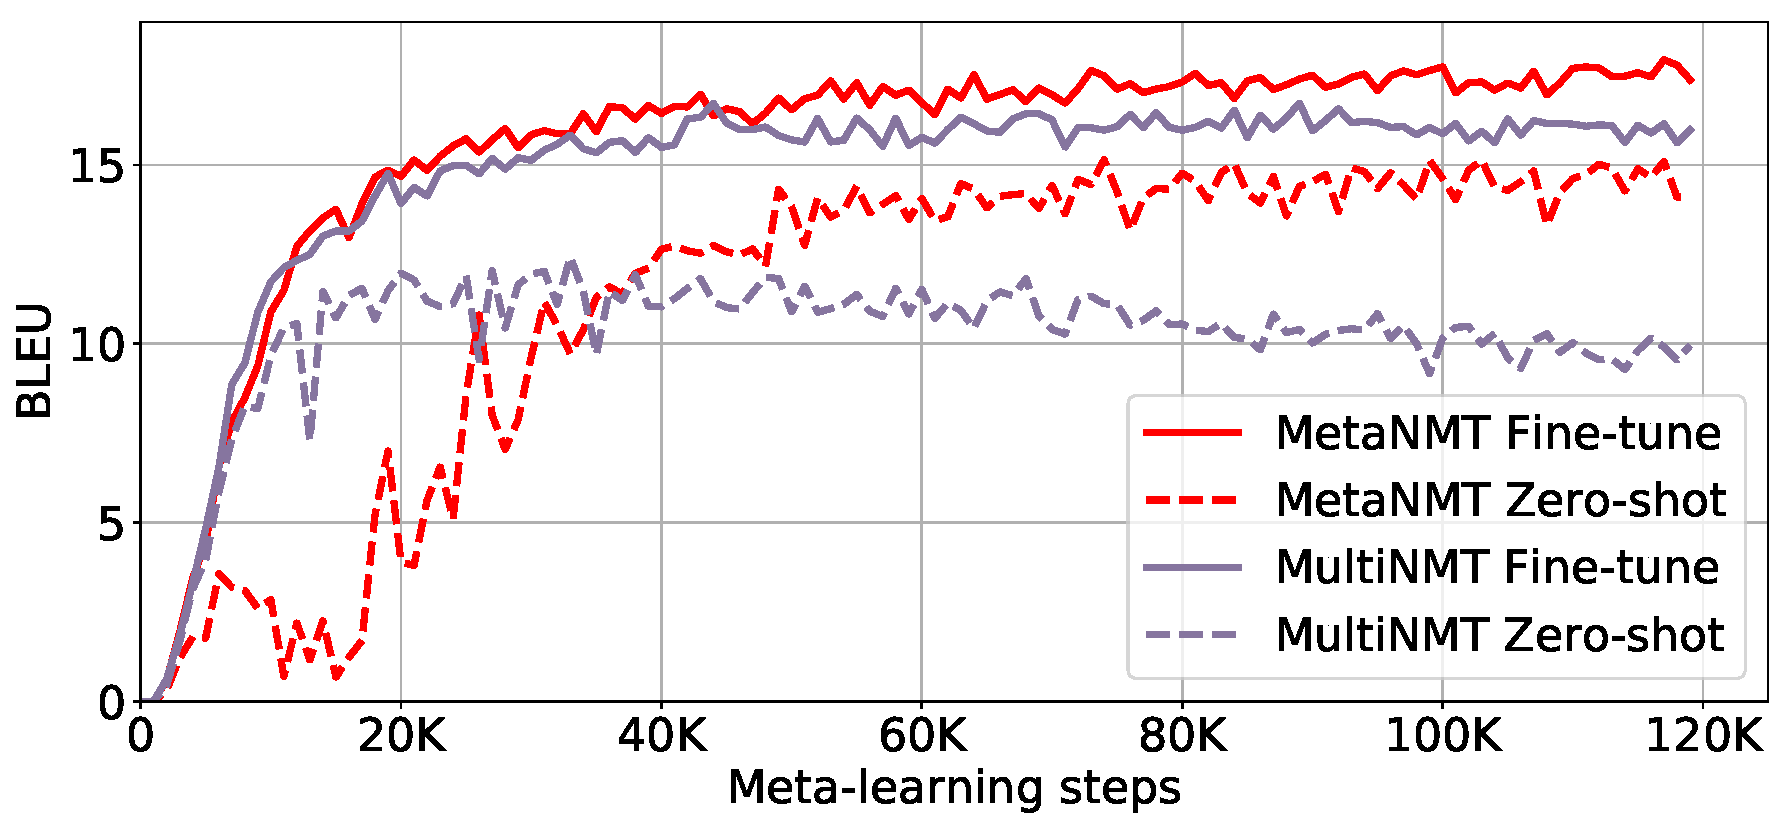
\includegraphics[width=0.8\linewidth]{figs/meta/curve.pdf}
    \caption{The learning curves of BLEU scores on the validation task (Ro-En).}%\alert{which target language pair?}}
    \label{cp6.fig.train_curve}
\end{figure}

\begin{sidewaystable}[hptb]
\centering
\resizebox{\textheight}{!}{
\begin{tabular}{l|cc|cc|cc|cc|cc}
\toprule
\multirow{2}{*}{Meta-Train} &  \multicolumn{2}{c|}{Ro-En} & \multicolumn{2}{c|}{Lv-En} & \multicolumn{2}{c|}{Fi-En} & \multicolumn{2}{c|}{Tr-En} & \multicolumn{2}{c}{Ko-En}\\
& zero & finetune & zero & finetune &  zero & finetune & zero & finetune & zero & finetune \\
\midrule
$-$                               &&$00.00 \pm .00$& & $0.00 \pm .00$  &  &$0.00 \pm .00$ & &$0.00 \pm .00$ & &$0.00 \pm .00$\\
Es                                &$9.20$&$15.71 \pm .22$& $2.23$& $4.65 \pm .12$  &  $2.73$&$5.55 \pm .08$ & $1.56$&$4.14 \pm .03$ & $0.63$&$1.40 \pm .09$\\
Es Fr                             &$12.35$&$17.46 \pm .41$& $2.86$& $5.05 \pm .04$  &  $3.71$&$6.08 \pm .01$ & $2.17$&$4.56 \pm .20$ & $0.61$&$1.70 \pm .14$ \\
Es Fr It Pt                       &$13.88$&$18.54 \pm .19$& $3.88$& $5.63 \pm .11$  &  $4.93$&$6.80 \pm .04$ & $2.49$&$4.82 \pm .10$ & $0.82$&$1.90 \pm .07$\\
\quad \quad \quad \quad\, De Ru   &$10.60$&$16.05 \pm .31$& $5.15$& $7.19 \pm .17$  &  $6.62$&$7.98 \pm .22$ & $3.20$&$6.02 \pm .11$ & $1.19$&$2.16 \pm .09$ \\
Es Fr It Pt De Ru                 &$15.93$&$20.00 \pm .27$& $6.33$& $7.88 \pm .14$  &  $7.89$&$9.14 \pm .05$ & $3.72$&$6.02 \pm .13$ & $1.28$&$2.44 \pm .11$ \\
All                &$18.12$&$\bm{22.04 \pm .23}$& $9.58$& $\bm{10.44 \pm .17}$ &  $11.39$&$\bm{12.63 \pm .22}$ & $5.34$ &$\bm{8.97 \pm .08}$ & $1.96$&$\bm{3.97 \pm .10}$ \\
\midrule
Full Supervised                   & \multicolumn{2}{c|}{$31.76$}& \multicolumn{2}{c|}{$15.15$} & \multicolumn{2}{c|}{$20.20$} & \multicolumn{2}{c|}{$13.74$} & \multicolumn{2}{c}{$5.97$}\\
\bottomrule
\end{tabular}
}
\caption{\label{cp6.table.aux}
BLEU Scores w.r.t. the source task set for all five target tasks.}
\end{sidewaystable}
\begin{table*}[hptb]
\centering
\small
%\resizebox{\textwidth}{!}{
\begin{tabular}{p{0.1\textwidth}|p{0.81\textwidth}}
\toprule
Source (Tr) & google \textcolor{blue}{mülteciler} için 11 milyon dolar \textcolor{purple}{toplamak} üzere bağış eşleştirme \textcolor{orange}{kampanyasını} \textcolor{red}{başlattı} .\\
Target & google \textcolor{red}{launches} donation-matching \textcolor{orange}{campaign} to \textcolor{purple}{raise} \$ 11 million for \textcolor{blue}{refugees} .\\
%Multi & \\
Meta-0 & google \textcolor{blue}{refugee} \textcolor{purple}{fund} for usd 11 million has \textcolor{red}{launched} a \textcolor{orange}{campaign} for donation .\\
Meta-16k & google has \textcolor{red}{launched} a \textcolor{orange}{campaign} to \textcolor{purple}{collect} \$ 11 million for \textcolor{blue}{refugees} . \\
\midrule
Source (Ko) & 이번에 체포되어 기소된 사람들 중에는 퇴역한 군 고위관리 , 언론인 , 정치인 , 경제인 등이 \textcolor{blue}{포함됐다} \\
Target & \textcolor{blue}{among} the suspects \textcolor{blue}{are} retired military officials , journalists , politicians , businessmen and others .\\
%Multi & \\
Meta-0 & last year , convicted people , among other people , of a high-ranking army of journalists in economic and economic policies , \textcolor{blue}{were included} . \\
Meta-16k & the arrested persons \textcolor{blue}{were included} in the charge , \textcolor{blue}{including} the military officials , journalists , politicians and economists .\\
% \midrule
% \midrule
% Source (Ro) & astfel , lucrarile de consolidare a cladirii ar putea fi reluate cel mai devreme anul viitor .\\
% Target & thus , the consolidation of the building could resume as early as next year .\\
% Multi & thus , building building building building building building could be resumed before next year .\\
% %Meta-0 & \\
% Meta-16k & thus , the building of the building could therefore be resumed as early as next year .\\
\bottomrule
\end{tabular}
%}
\caption{\label{cp6.table.example}
Sample translations for Tr-En and Ko-En highlight the impact of fine-tuning which results in syntactically better formed translations. We highlight tokens of interest in terms of reordering.
}
% KC: the last example is not too informative. a similar issue would be easily found with any kind of translation system.
% In the last example, we 
% Tr-En and Ko-En compare the difference of zero-shot and finetune, while Ro-En compares the difference of MetaNMT and MultiNMT. The same color denotes the same meanings.}
\end{table*}



\paragraph{Impact of Source Tasks}
In Table~\ref{cp6.table.aux}, we present the results on all five target tasks obtained while varying the source task set. We first see that it is always beneficial to use more source tasks. Although the impact of adding more source tasks varies from one language to another, there is up to 2$\times$ improvement going from one source task to 18 source tasks (Lv-En, Fi-En, Tr-En and Ko-En). The same trend can be observed even without any fine-tuning (i.e., unsupervised translation, \citep{lample2017unsupervised,artetxe2017unsupervised}). In addition, the choice of source languages has different implications for different target languages. For instance, Ro-En benefits more from \{Es, Fr, It, Pt\} than from \{De, Ru\}, while the opposite effect is observed with all the other target tasks. 


\paragraph{Training Curves}

The benefit of meta-learning over multilingual translation is clearly demonstrated when we look at the training curves in Fig.~\ref{cp6.fig.train_curve}. With the multilingual, transfer learning approach, we observe that training rapidly saturates and eventually degrades, as the model overfits to the source tasks. MetaNMT on the other hand continues to improve and never degrades, as the meta-objective ensures that the model is adequate for fine-tuning on target tasks rather than for solving the source tasks.

\paragraph{Sample Translations}
We present some sample translations from the tested models in Table~\ref{cp6.table.example}. Inspecting these examples provides the insight into the proposed meta-learning algorithm. For instance, we observe that the meta-learned model without any fine-tuning produces a word-by-word translation in the first example (Tr-En), which is due to the successful use of the universal lexcial representation and the meta-learned initialization. The system however cannot reorder tokens from Turkish to English, as it has not seen any training example of Tr-En. After seeing around 600 sentence pairs (16K English tokens), the model rapidly learns to correctly reorder tokens to form a better translation. A similar phenomenon is observed in the Ko-En example. These cases could be found across different language pairs.  


% Then, we can see that MetaNMT outperforms MultiNMT evidently in qualitative results. For example, for Ro-En, MetaNMT can translate this sentence properly comforming to English grammar and using suitable words and phrases while MultiNMT fails to do this.







% \subsection{Quantitative Comparison}

% We first conduct the experiments and evaluate the performance of metaNMT and multilingual transfer learning (MultiNMT) with a fixed training set which consists of six source tasks: Es Fr It Pt De Ru. Four target datasets (Ro Lv Fi Tr) with 16K En tokens are selected for the initial experiments.

% \paragraph{Overall performance}


% \paragraph{Fine-tuning St}
% Following \cite{zoph2016transfer}, fine-tuning different modules is investigated, namely finetune all, freeze decoder and only finetune embedding. Freeze decoder means that we finetune embedding and encoder. The main results are shown in Fig. \ref{cp6.fig.compare}. Here, we use the language sentences pairs which have $16,000$ En tokens. Firstly, it is very obvious that MetaNMT outperforms MultiNMT in all language pairs and finetune different modules. Secondly, when we only finetune encoder embedding, the improvements are the best among the three schemes of fine-tuning different modules. Especially, for Ro-En, MetaNMT can improve from $14.25$ to $18.34$ for Ro-En valication. Thirdly, the choice of validation set is very important and it affects the results greatly. If we use Ro-En as validation set, the improvements will be greater than choose Lv-En as validation set.  Fourthly, for different language pair, the improvements of performance are different. For Tr-En, the improvements are very small contrast to the great improvements for Ro-En.  
% \paragraph{v.s. support size}
% We also investigate the improvements as the increase of size of support sets. The results are shown in Fig. \ref{cp6.fig.support}. Firstly, we can see that when the size of support sets increases, the performance of MetaNMT and MultiNMT will increase. Secondly, when the size of support sets is very small, MetaNMT outperforms MultiNMT greatly. Especially, for Ro-En, when the size of support sets is $0$, MetaNMT can improve the performance from $11.55$ to $16.13$ than MultiNMT. Thirdly, when the size of support sets increases to a certain amount, the performance of MetaNMT and MultiNMT will have almost no difference. However, the performance of MetaNMT is always better than MultiNMT. For different language pairs, the observed results are the same.





% \paragraph{v.s. meta-learn languages}
% We also investigate the influence of using different language pairs in meta-train. The results are shown in Table \ref{cp6.table.aux}. Firstly, when more language pairs are added to the meta-train languages, the performance of both zero and finetune setting will increase. For example, after we add Fr to the source languages, the performance will be improved. When we use full Europarl and Ru as our meta-train dataset, the performance of finetune will achieve $22.04$ which has a very competitive performance contrast to full supervised setting. Secondly, for different target language pairs, different source language pairs will help them differently. For example, when the source languages change from Es Fr It Pt to De Ru, the performance of Ro-En drops from $18.54$ to $16.05$ while the performances of Lv-En, Fi-En, Tr-En and Ko-En all rise.



\section{Conclusion and Next Chapter}

In this chapter, we proposed a meta-learning algorithm for low-resource neural machine translation that exploits the availability of high-resource language pairs. We based the proposed algorithm on the recently proposed model-agnostic meta-learning and adapted it to work with multiple languages that do not share a common vocabulary using the technique of universal lexical representation, resulting in MetaNMT. Our extensive evaluation, using 18 high-resource source tasks and 5 low-resource target tasks, has shown that the proposed MetaNMT significantly outperforms the existing approach of multilingual, transfer learning in low-resource neural machine translation across all the language pairs considered.

The proposed approach opens new opportunities for neural machine translation. First, it is a framework for incorporating various extra sources of data, such as source- and target-side monolingual corpora. Second, it is a generic framework that can easily accommodate existing and future neural machine translation systems. 

Up to now we have basically introduced one direction of achieving a data-efficient neural machine translation system. From the next chapter, we will further investigate another important component of the existing NMT, i.e., decoding. We will first start to introduce a general learning framework -- {\it trainable decoding} --which can learn to build a decoding-efficient NMT system.